
\section{Evaluation}
\label{sec:ev}

In this section, we analyze the performance of the \pnum~protocols that we have implemented over \odlib.
% Whenever necessary, we will discuss modifications the protocols to improve their thread-scalability, implement reads and match them with the KVS. We will discuss such modifications as we go along.
We start the discussion by providing a high-level overview of the 
%performance of the protocols. 
key insights of this evaluation.
Then we individually analyze the performance of each class of protocols. 
%In \secref{sec:ev:mcast}, we describe the impact of the hardware multicast primitive (introduced in \S\ref{sec:nw:mcast}).

\subsection{Overview} 
% (\figref{fig:three-bars} \& \tabref{tab:all-perf})}
\label{sec:ev:ov}

\begin{figure*}[t]
\centering
  \begin{subfigure}[b]{0.33\textwidth}
    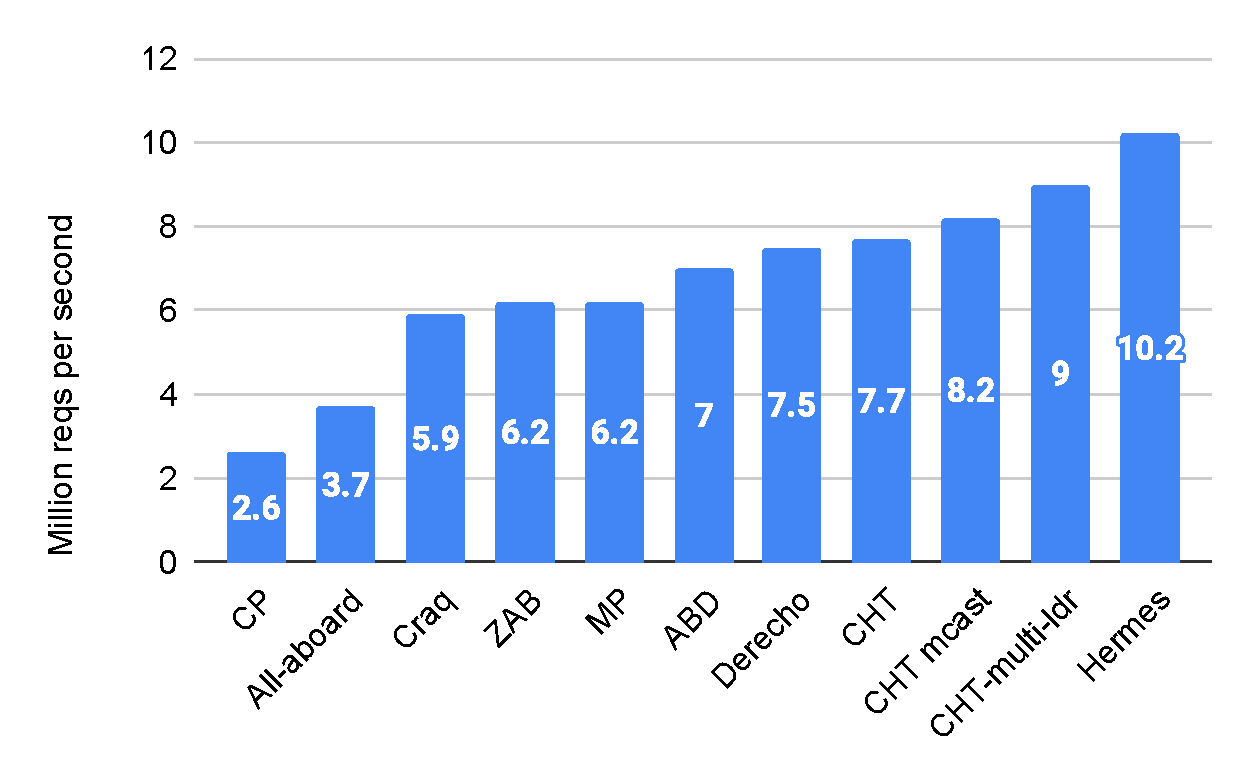
\includegraphics[width=\textwidth]{1_figures/single-thread.pdf}
    % \captionsetup{width=0.85\linewidth}
    % \vspace{-1.8em}
    \caption{Single-threaded write throughput}
%   \vspace{-1.5em}
  \label{fig:single-thr}
  \end{subfigure}
  %
  \begin{subfigure}[b]{0.33\textwidth}
    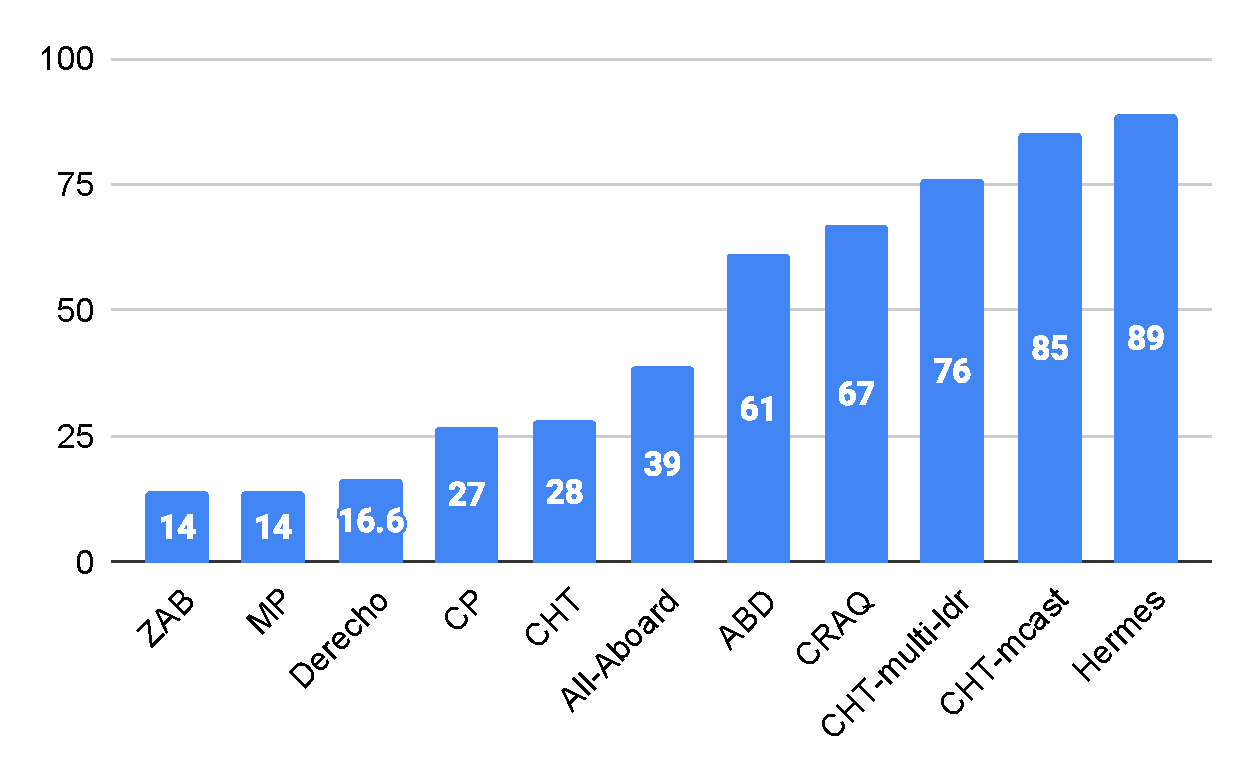
\includegraphics[width=\textwidth]{1_figures/Write-only-chart.pdf}
    % \captionsetup{width=0.85\linewidth}
    % \vspace{-1.8em}
    \caption{Multi-threaded write throughput}
    %   \vspace{-1.5em}
  \label{fig:write-all}
  \end{subfigure}
  %
  \begin{subfigure}[b]{0.33\textwidth} 
  
    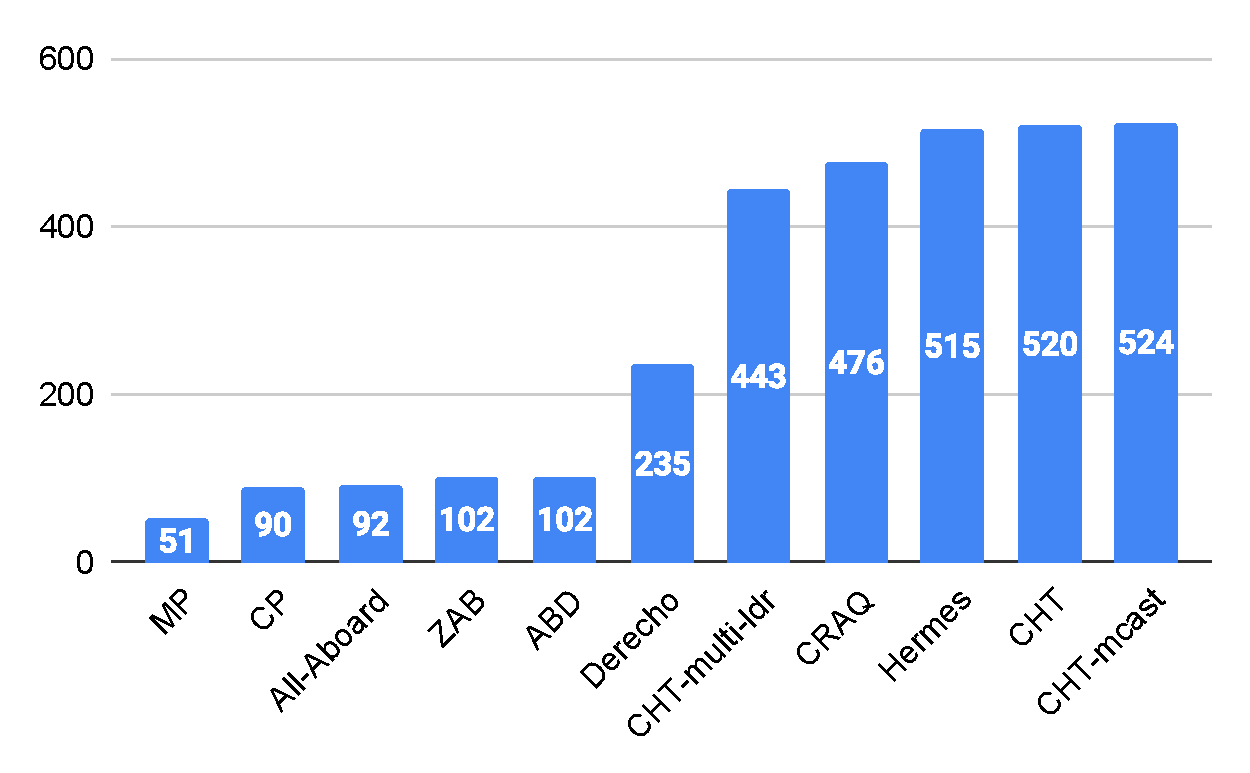
\includegraphics[width=\textwidth]{1_figures/5perc-writes.pdf}
    % \captionsetup{width=0.85\linewidth}
    % \vspace{-1.8em}
    \caption{Multi-threaded throughput at 95\% reads}
%   \vspace{-1.5em}
  \label{fig:5perc}
  \end{subfigure}
%   \vspace{-1em}
  \caption{Throughput comparison of all protocols in M.reqs/s. Note that both the x-axes and y-axes are different in each graph.}
 %\antonis{caption is closer to the text below than the subcaptions above}}
  \label{fig:three-bars}
%   \vspace{-1em}
\end{figure*}
% \begin{figure*}[t]
\centering
  \begin{subfigure}[b]{0.33\textwidth}
    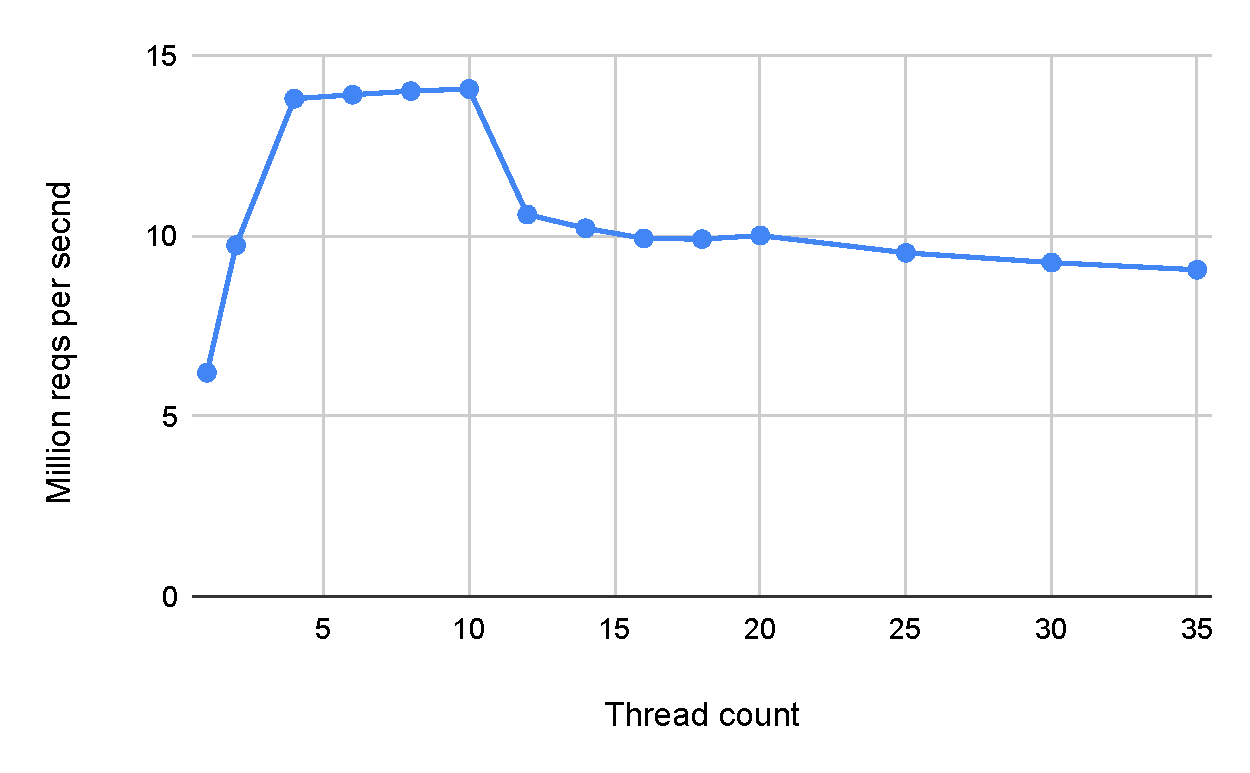
\includegraphics[width=\textwidth]{1_figures/ZAB-scal.pdf}
    \captionsetup{width=0.85\linewidth}
    % \vspace{-1.8em}
    \caption{Write-only throughput vs. thread cound for ZAB and MP}
%   \vspace{-1.5em}
  \label{fig:zab-scal}
  \end{subfigure}
  %
  \begin{subfigure}[b]{0.33\textwidth}
    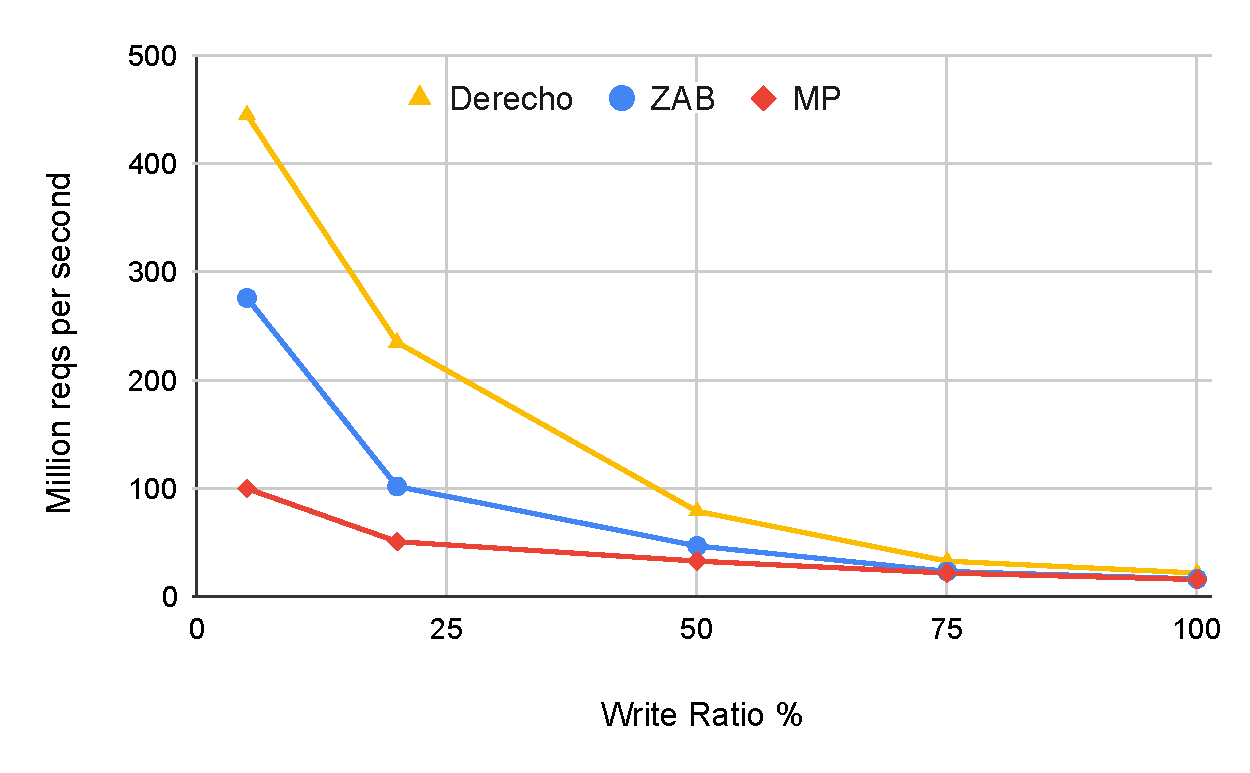
\includegraphics[width=\textwidth]{1_figures/zab-mp-dr.pdf}
    \captionsetup{width=0.85\linewidth}
    % \vspace{-1.8em}
    \caption{Throughput vs. write ratio for ZAB, MP \& Derecho}
    % \vspace{-1.5em}
  \label{fig:zab-mp-dr}
  \end{subfigure}
  %
  \begin{subfigure}[b]{0.33\textwidth} 
  
    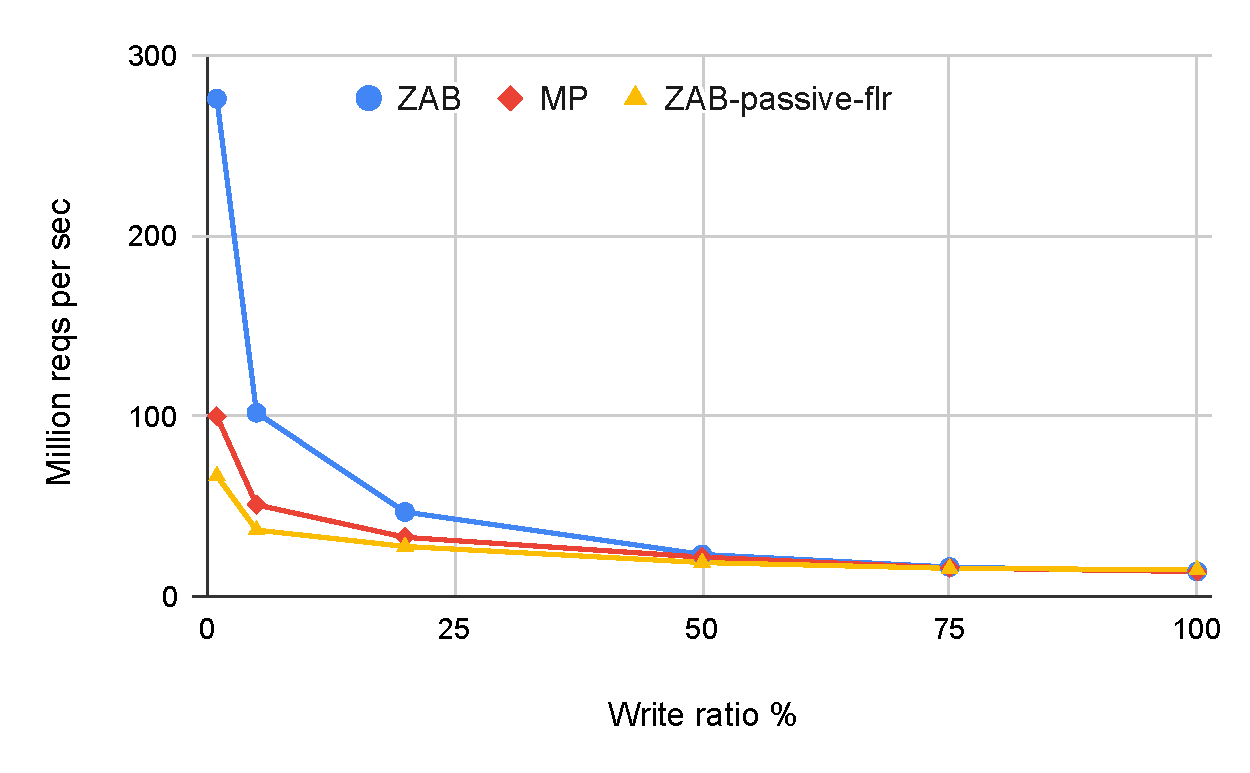
\includegraphics[width=\textwidth]{1_figures/zab-passive-flr.pdf}
    % \captionsetup{width=0.85\linewidth}
    \vspace{-1.8em}
    \caption{Throughput vs. write ratio for ZAB, MP and ZAB/MP with passive followers}
%   \vspace{-1.5em}
  \label{fig:zab-psv}
  \end{subfigure}
%   \vspace{-1em}
  \caption{Comparing ZAB, MP \& Derecho}
  \label{fig:lto}
%   \vspace{-1em}
\end{figure*}


% \begin{figure*}[t]
% \centering

% \begin{subfigure}[b]{0.33\textwidth}
%     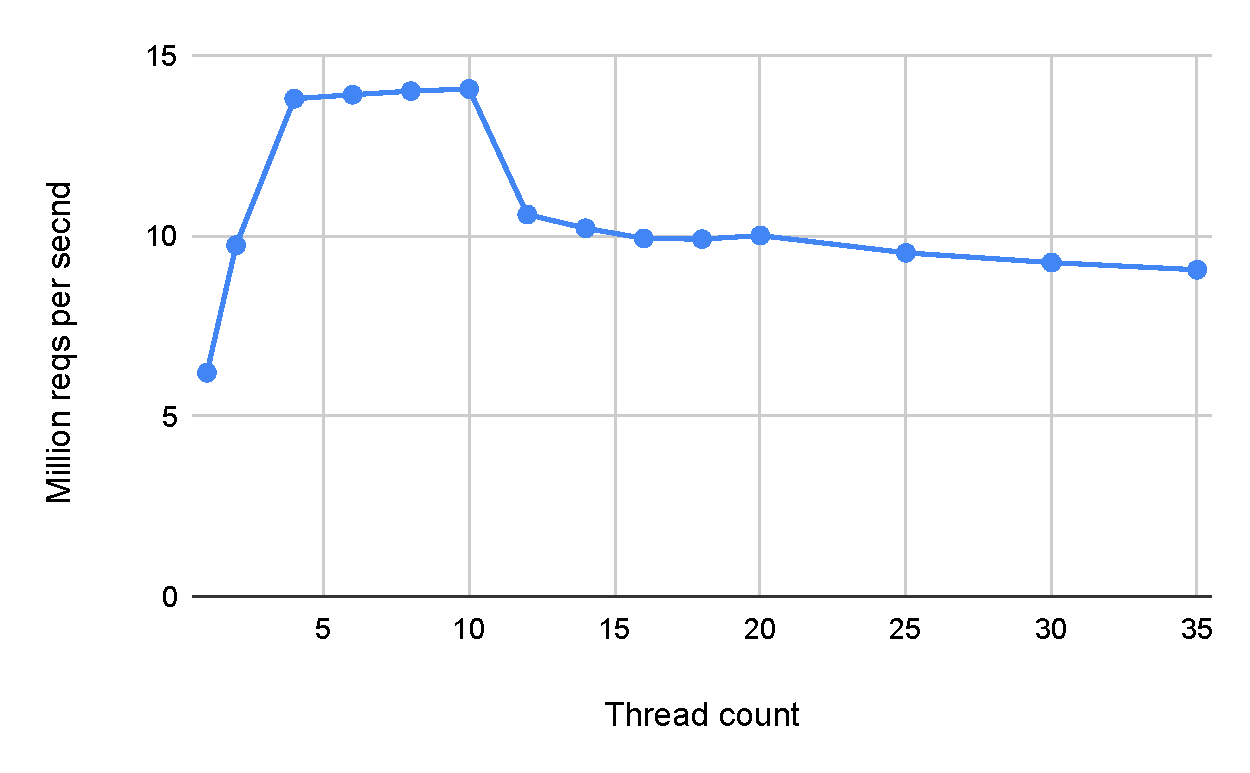
\includegraphics[width=\textwidth]{1_figures/ZAB-scal.pdf}
%     % \captionsetup{width=0.85\linewidth}
%     % \vspace{-1.8em}
%   \caption{Write-only throughput of ZAB and MP, varying the workers}
% %   \vspace{-1.5em}
%   \label{fig:zab-scal}
%   \end{subfigure} %%
  
% \begin{subfigure}[b]{0.33\textwidth}
% 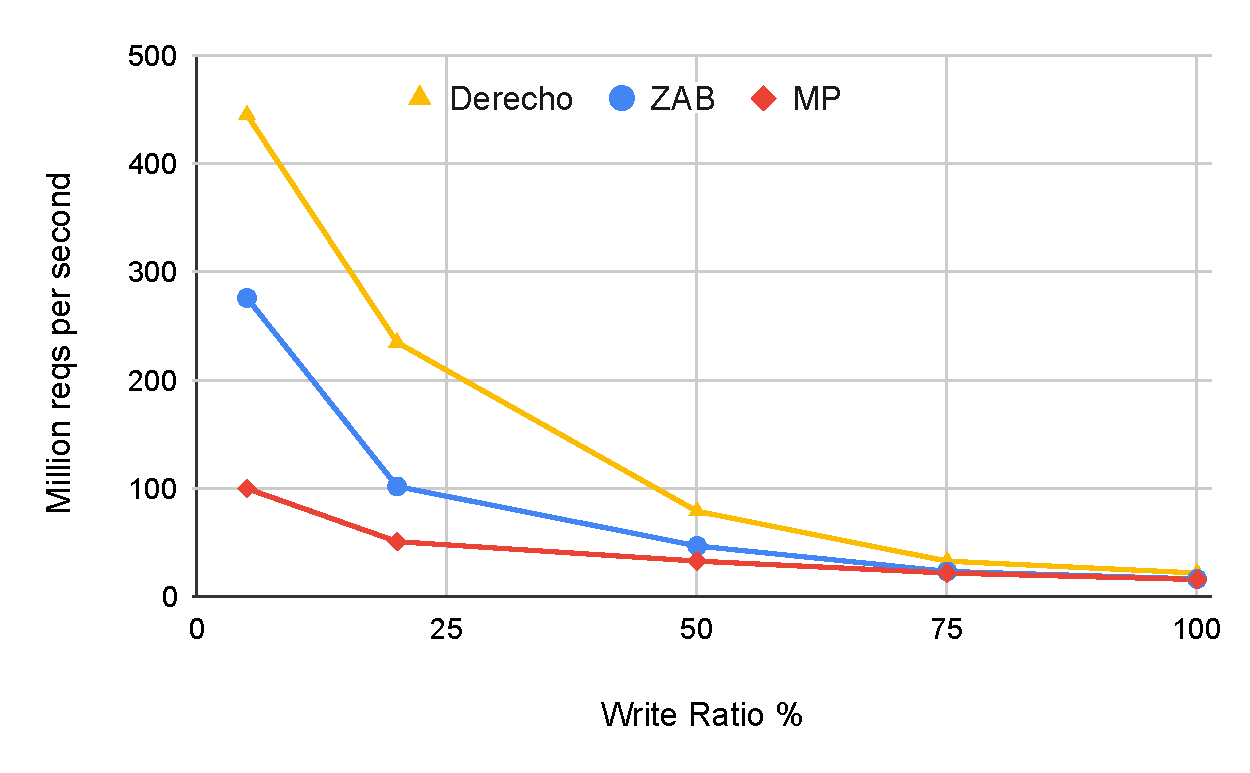
\includegraphics[width=\textwidth]{1_figures/zab-mp-dr.pdf}
% % \captionsetup{width=0.85\linewidth}
% % \vspace{-1.8em}
% \caption{Throughput of ZAB, MP \& Derecho, varying the write ratio from 1\% to 100\%}
% %   \vspace{-1.5em}
% \label{fig:zab-mp-dr}
% \end{subfigure}%

% \begin{subfigure}[b]{0.33\textwidth} 

% 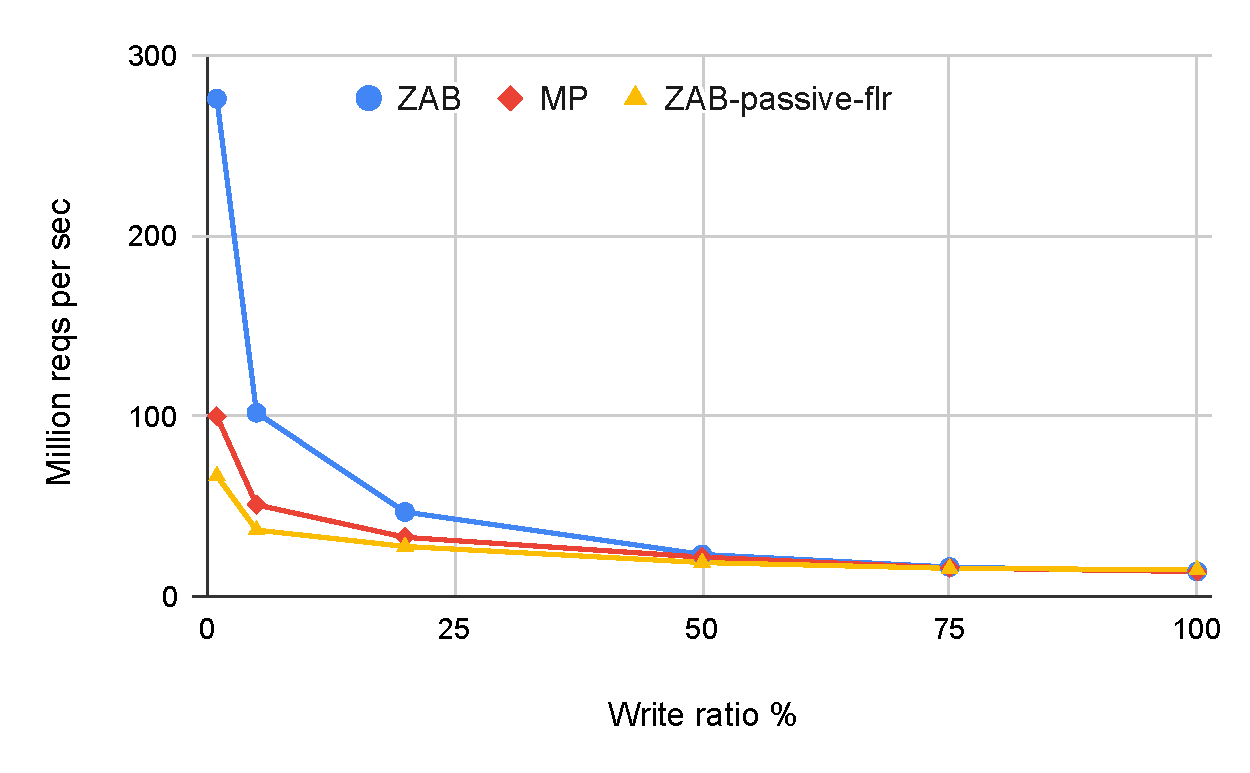
\includegraphics[width=\textwidth]{1_figures/zab-passive-flr.pdf}
% %   \vspace{-0.5em}
% \caption{Throughput of ZAB, MP and ZAB/MP with passive followers, when varying the write ratio}
% %   \vspace{-1.5em}
% \label{fig:zab-psv}
% \end{subfigure}%
% %   \vspace{-2em}
% \caption{\LTO~graphs. }
% \label{fig:lto}
% %   \vspace{-1.5em}
% \end{figure*}

First, we briefly describe \figref{fig:three-bars} and \tabref{tab:all-perf} and then analyze our key insights and provide general directives and recommendations. 

\beginbsec{\figref{fig:three-bars}}
\figref{fig:three-bars} shows the throughput of all protocols in million requests per second (M.reqs/s), ordering the protocols in ascending throughput order. 
% \figref{fig:single-thr} shows the order when the protocol are single-threaded, \figref{fig:write-all} when they are multi-threaded (the default case), and 
Specifically, \figref{fig:single-thr} and \ref{fig:write-all} show the write throughput of the protocols when they are single-threaded and multi-threaded (default scenario), respectively.
% \figref{fig:write-all} shows the same write throughput when protocols are multi-threaded (default scenario).
Finally, \figref{fig:5perc} shows the throughput (multi-threaded), with 95\% reads.




Note the following three remarks for \figref{fig:three-bars}.
Firstly, both the x-axis and y-axis are different in all three graphs. Crucially, protocols in the x-axis are ordered in ascending throughput order.
% to highlight their performance relation
Secondly, MP and ZAB are the same protocol in the write-only workload, \ie in \figref{fig:single-thr} and \ref{fig:write-all}, because they only differ in the execution of reads.
Third and final, note that there is a protocol called \emph{CHT-mcast}: this is the CHT protocol with the hardware multicast enabled. We show its performance separately because it performs significantly better than CHT. Enabling the multicast in the rest of the protocols has a very small impact. %, and we discuss why in Section~\secref{sec:ev:mcast}.

\beginbsec{\tabref{tab:all-perf}}
The left-hand side of \tabref{tab:all-perf} shows the throughput in M.reqs/s of all protocols when varying the write ratio. 
% Throughout this section, we plot the throughput measurements from this table whenever necessary.
The right-hand side shows the latency (99th / average) of all protocols in microseconds at 100\% write ratio, while varying the load of the protocol (\ie with respect to peak throughput). 
% In ZAB, MP and CHT variants, we have measured the latency at a follower node. In CRAQ, we have measured the latency at the head node.

\custvspace
\noindent
Let us now summarize the key insights from this study.

% \beginbsec{Observations}

\beginbsec{1. Total order is not thread-scalable}
Protocols that apply writes in a total order are not thread-scalable:
the relative positions of ZAB, MP (\LTO), and Derecho (\DTO) in \figref{fig:single-thr} and \figref{fig:write-all} demonstrate this point. The reason is that explicitly enforcing total order mandates that threads can only apply writes to the KVS in lock-step.
In contrast, protocols that enforce per-key order (\LPKO~and \DPKO) can scale well with more threads.

\beginbsec{2. The leader jeopardizes load balance}
The adverse effect of the leader on load balance is not apparent in \LTO~protocols because they cannot scale enough to uncover it.
However it is visible in \LPKO~protocols.
% \LPKO~protocols, struggle to achieve load balance. 
Specifically, CHT does not scale well when multi-threaded because the send side of the leader becomes the bottleneck. % as the leader is responsible for broadcasting every write.
There are two protocol-level optimizations that restore load balance: propagating writes through a chain (\ie CRAQ) and using multiple leaders (\ie CHT-multi-ldr).
% Finally, we expose a third optimization using the hardware multicast primitive (\ie CHT-mcast). In \secref{sec:}, we explain how multicast makes a leader-based protocol as efficient as a decentralized protocol such as Hermes.

\beginbsec{3. Hardware multicast is effective for \LPKO}
The hardware multicast primitive can make a huge difference, but only in \LPKO~protocols.
Specifically, the hardware multicast primitive provides a 3x benefit for CHT, i.e., CHT-mcast. 
The benefit for the rest of the protocols is very small, typically around 5\%.
The reason is that the multicast only relieves load on the send side of the node that performs the broadcast: it reduces the number of messages sent, but not the number of messages received.
Therefore, multicast is extremely useful for leader-based protocols that are bottlenecked by the send bandwidth of the leader. It is not so useful for already well-balanced protocols (\ie \DTO\  and \DPKO), while \LTO\ protocols do not benefit, as they are already bottlenecked by thread-scalability. We will expand in \secref{sec:ev:lpko}.% This is highlighted by the performance of CHT-mcast, which removes that bottleneck by using the multicast primitive.
% CRAQ and CHT-multi-ldr which explicitly target load balance also achieve very good performance.

\beginbsec{4. \DPKO~excels when multi-threaded}
In the absence of a leader or a total order, \DPKO\ protocols must find creative ways to serialize writes in a decentralized manner.
% \DPKO~protocols have a high work-per-request ratio, because in the absence of a leader or a total order, they must find creative ways to serialize writes.
On the one hand, this invites a level of complexity that has an adverse affect on the work-per-request ratio. 
This is portrayed by the single-threaded performance of CP and All-Aboard, which is the lowest among all protocols.
On the other hand, the decentralized nature of these protocols makes them
naturally thread-scalable and load balanced. This is why multi-threading yields a $\sim$9-10x throughput improvement.
Notably, by downgrading the availability guarantees, as in Hermes, or downgrading the API, as in ABD, it is possible reduce the work-per-request ratio.

\beginbsec{5. Thread-scalability > load balance > work-per-request}
From \figref{fig:write-all}, we observe that the non-thread-scalable protocols, ZAB, MP and Derecho are the worst performers, rendering thread-scalability the most critical property to honour in the modern era.
Furthermore, All-Aboard, a protocol with a very high work-per-request ratio, significantly outperforms CHT, which sacrifices load balance, even though CHT offers lower availability guarantees (discussed in \S\ref{sec:fail}).
From that we concur that it is preferable to optimize for load balance rather than work-per-request ratio. At the limits of the work-per-request ratio (\ie in CP), the two metrics appear equally important, as CHT and CP are roughly matched.



% However, \DPKO~protocols are also naturally thread-scalable and load balanced, which is why multi-threading yields a $\sim$9-10x throughput improvement---making CP, All-aboard, and ABD attractive design points for systems keen on favouring availability. 
% Hermes is the best-performing protocol in both \figref{fig:single-thr} and~\ref{fig:write-all}.
% That is because
% Hermes keeps the work-per-request low by mandating that every message must reach all machines. The cost of this choice is an availability penalty in case of a failure.

\beginbsec{6. Local reads are great but with caveats}
Recall that MP performs reads by sending them to the leader. CP, All-aboard and ABD perform ABD-reads (typically 1 broadcast round). The rest perform reads locally.
From \figref{fig:5perc}, we see that there is a big gap between protocols with local reads and the rest, which perform them remotely. However there are a couple of caveats.
Firstly, local reads always come at a cost as they downgrade either the consistency or the availability guarantees, as we saw in \secref{sec:fail}.
Furthermore, note that ZAB, even though it performs its reads locally, is on par with the protocols that perform reads remotely.
This is because it is bottlenecked by its write throughput.
We elaborate in \secref{sec:ev:lto}.
% Specifically, since ZAB's peak write throughput is 14 M.reqs/s, that means that its theoretical limit at 5\% writes is 280 M.reqs/s. In practice, ZAB reaches only 102 M.reqs/s
% The conclusion is that local reads are extremely beneficial, however, they can be bottlenecked by the write throughput in protocols that do not scale well.

% In fact, in the modern era we argue that the opposite is true: in order to optimize latency, one should actually prioritize thread-scalability and load balance.
% Here is why. With networking and memory accounting for a few microseconds, the request latency does not typically exceed a few tens of microseconds on a lightly loaded system. 
% Therefore, to ensure microsecond latency, we need only ensure that the system is not overloaded.
% This calls for high-throughput protocols as the target throughput is less likely to overload such protocols. 
% To maximize throughput,  thread-scalability and load balance should be prioritized over traditional metrics such as number of messages per request.
% Our evaluation corroborates this hypothesis (\S~\ref{sec:ev}).

\beginbsec{7. For better latency, choose throughput}
In the Introduction, we hypothesized that a request's latency should not exceed a few tens of microseconds in a lightly loaded system. 
Furthermore, we argued that to ensure a low latency, we should favour high-throughput protocols. %, as they will be less loaded at the target throughput.
The latency measurements for 25\% load in \tabref{tab:all-perf} verify that at a light load, all protocols incur a latency of a few tens of microseconds. 
Furthermore, we observe that for all protocols, as load increases so does latency, with a big spike at 100\% load. Therefore, to maintain a latency of a few tens of microseconds, 
%we need to ensure the protocol is not overloaded.
% To achieve that, 
one should favour high-throughput protocols, as they will be less likely to be overloaded when operating on the target throughput. %, and thus more likely to deliver a lower latency.
% In fact, using 
% In all cases, going from 25\% load to 75\% or 100\%  has a worse effect in latency than 
% %at a light load.
% All protocols see a big jump in latency when 100\% loaded.
% % However, for all protocols, as load increases so does latency.
% Therefore, to achieve the lowest latency, one should favour high-throughput protocols, as they will be less loaded when operating on the target throughput, and thus more likely to deliver a lower latency.
% For example, Hermes achieves roughly the same throughput at 25\% load as ZAB does at 100\% load.  but enjoying a significantly lower latency.
% For that reason
% Therefore, the protocol with the lowest load at the target throughput is the most likely to achieve the lowest latency. 
% Therefore, even when optimizing for latency, one should favour throughput, as high-throughput protocols will be less loaded at the target throughput.

% Note, however that Hermes achieves higher throughput at 25\% load than ZAB at 100\% load. Therefore, for the same throughput requirements, Hermes will enjoys a lower latency, simply because it is less loaded.
% This corroborates our hypothesis that for better latency, high-throughput protocols should be favoured.
% Furthermore, we argued that to maintain this low latency, we only needed to ensure that the system would not become overloaded. To achieve that we should favour high-throughput protocols, as they will be less loaded at the target throughput. Again, from 


% From the latency results in \tabref{tab:all-perf} we make the following observation.
% There is not a strong correlation between the work-per-request ratio and the latency of the protocols. Instead, the most impactful factor is the load imposed on a protocol. Specifically, all protocols incur a few microseconds at 25\% load, which grows to 100s of microseconds at 100\% load. 
% It is crucial to note that protocols with the same load achieve different throughput.
% For instance, Hermes achieves a higher throughput at 25\% load than ZAB at 100\% load. Therefore, for the same throughput requirements, Hermes enjoys a lower latency, simply because it is less loaded.
% Therefore, we recommend that a protocol is chosen based on its throughput capabilities. This will guarantee that the load on the protocol is always the lowest possible, which in turn yields the lowest latencies.


% \beginbsec{Conclusions}
% The conclusions of our evaluation are the following:
% Total order should always be avoided in read/write systems.
% Leader-based protocols can offer high-performance, but care must be taken to restore load balance.
% The hardware multicast primitive can make a huge difference but only in \LPKO~protocols.
% Local reads are very beneficial, but can be bottlenecked by the write throughput.
\beginbsec{Summary -- Recommendations}
Based on our insights, we first provide some general directives on protocol design and then offer recommendations on choosing a protocol.
% \fbox{
% \begin{minipage}{0.45 \textwidth}

\beginbsec{General Directives}
\squishlist
% Firstly, a few general directives.
\item %Among thread-scalability, load-balance and the work-per-request ratio, 
Prioritize thread-scalability, then load-balance and then the work-per-request ratio.
%Favouring thread-scalability is the most imporant concern. 
\item Total order should be avoided in read/write systems.
\item Leader-based protocols can achieve high-performance, but care must be taken to ensure load balance. 
\item It is worth investing in the hardware multicast primitive only in the case of \LPKO\ protocols. 
\item Local reads can deliver great performance, but it's not guaranteed.
%should be preferred for performance, but one should be wary of their cost.
\item In order to minimize latency, choose protocols with high throughput.
\squishend
% \beginbsec{Concrete Recommendations}
\noindent\textbf{Recommendations}
\squishlistContrib
\item All-aboard is the most attractive design point for a scenario where: 1) availability is the most important concern and 2) conditional writes are required.
\item If simple writes will do, then we recommend ABD.
\item If a small window of unavailability on a failure is tolerable, then Hermes is the best candidate, while CHT-multi-ldr and CRAQ are good alternatives.
\squishend 
% \end{minipage}
% }
\begin{comment}


\beginbsec{\tabref{tab:all-perf}: Throughput \& Latency}
The left-hand side of \tabref{tab:all-perf} shows the throughput in M.reqs/s of all \pnum~protocols (plus CHT-mcast) when varying the write ratio. 
Throughout this section, we plot the throughput measurements from this table whenever necessary.

The right-hand side shows the latency (99th / average) of all protocols in microseconds at 100\% write ratio, while varying the load of the protocol (\ie with respect to peak throughput). 
In ZAB, MP and CHT variants, we have measured the latency at a follower node. In CRAQ, we have measured the latency at the head node.
\end{comment}
\begin{comment}


\todo{I will write the part about latency, once i make another pass over the intro}
In \secref{sec:introduction}, we made a hypothesis and then based on that  a claim.
Our hypothesis was that 
there is not a strong correlation between the work-per-request ratio and the latency of the protocols. 
Our claim based on that was that the protocol designer should not try to minimize work-per-request at the expense of load balance or thread-scalability. Instead she should favour throughput in order to increase latency.

To test our hypothesis consider CP

It has the highest work-per-request ratio which includes three heavy broadcast rounds. 
However, its latency does not stand out. 
The reason is that with RDMA networking, sending a message takes only a few microseconds. 
However, the 99th percentile latency of CP at 100\% load is 216 microseconds. The dominant factor in that number is queuing. 
Queuing occurs as the request travels from buffer to buffer during its lifetime from the client thread to a worker thread, propagating to all nodes and coming back to the client. 

Now consider our claim. 
\end{comment}


\begin{figure*}[t]
\centering
  \begin{subfigure}[b]{0.33\textwidth}
    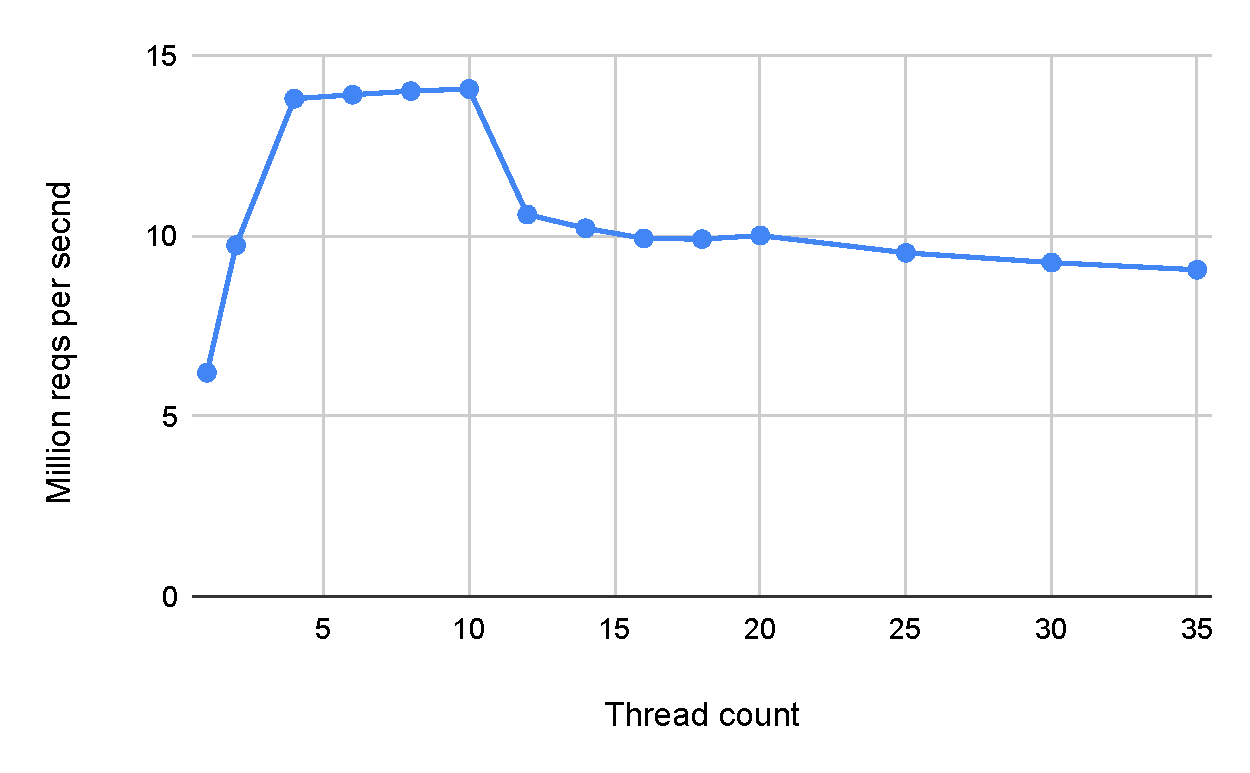
\includegraphics[width=\textwidth]{1_figures/ZAB-scal.pdf}
    \captionsetup{width=0.85\linewidth}
    % \vspace{-1.8em}
    \caption{Write-only throughput vs. thread cound for ZAB and MP}
%   \vspace{-1.5em}
  \label{fig:zab-scal}
  \end{subfigure}
  %
  \begin{subfigure}[b]{0.33\textwidth}
    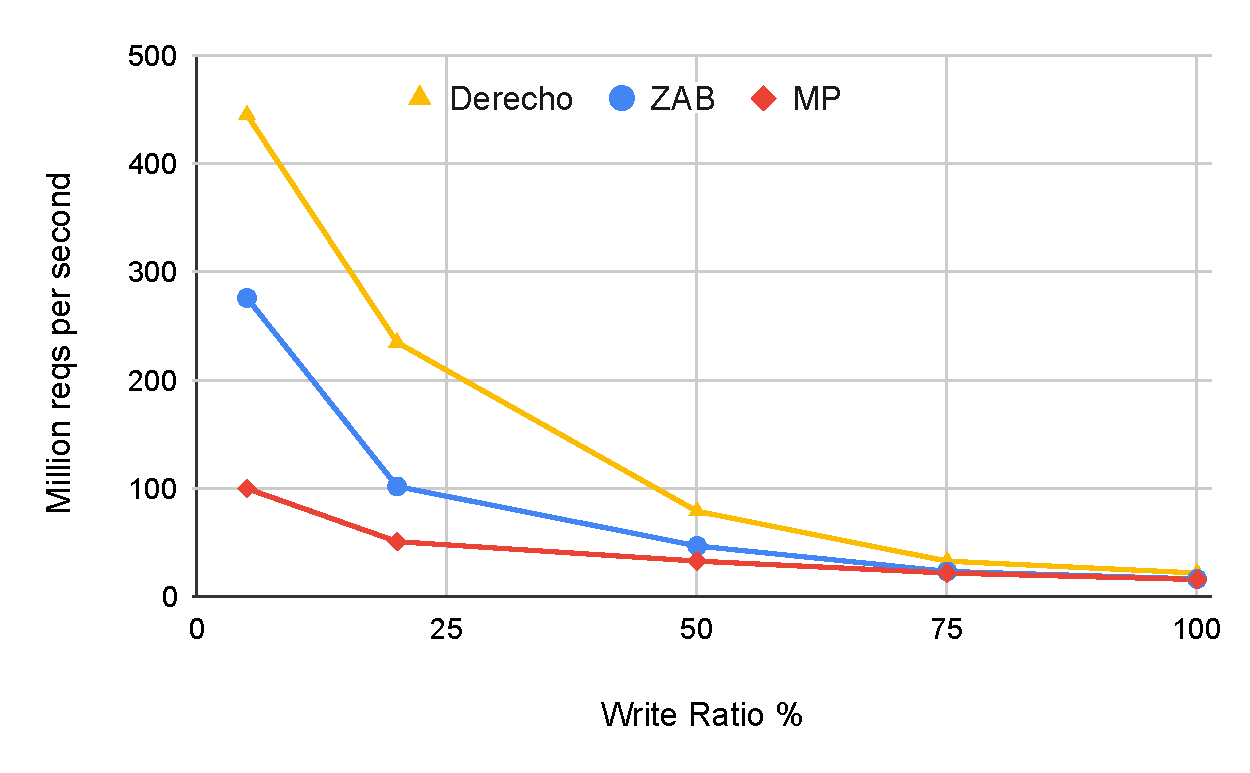
\includegraphics[width=\textwidth]{1_figures/zab-mp-dr.pdf}
    \captionsetup{width=0.85\linewidth}
    % \vspace{-1.8em}
    \caption{Throughput vs. write ratio for ZAB, MP \& Derecho}
    % \vspace{-1.5em}
  \label{fig:zab-mp-dr}
  \end{subfigure}
  %
  \begin{subfigure}[b]{0.33\textwidth} 
  
    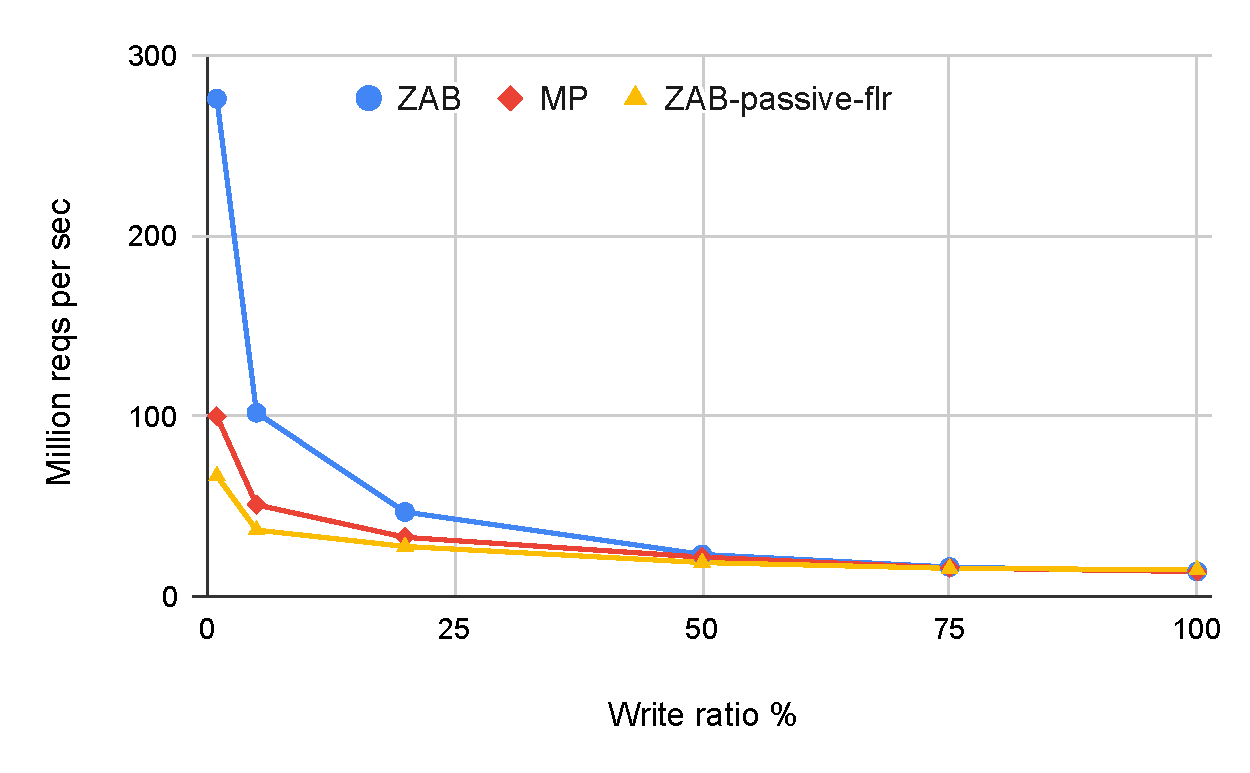
\includegraphics[width=\textwidth]{1_figures/zab-passive-flr.pdf}
    % \captionsetup{width=0.85\linewidth}
    \vspace{-1.8em}
    \caption{Throughput vs. write ratio for ZAB, MP and ZAB/MP with passive followers}
%   \vspace{-1.5em}
  \label{fig:zab-psv}
  \end{subfigure}
%   \vspace{-1em}
  \caption{Comparing ZAB, MP \& Derecho}
  \label{fig:lto}
%   \vspace{-1em}
\end{figure*}


% \begin{figure*}[t]
% \centering

% \begin{subfigure}[b]{0.33\textwidth}
%     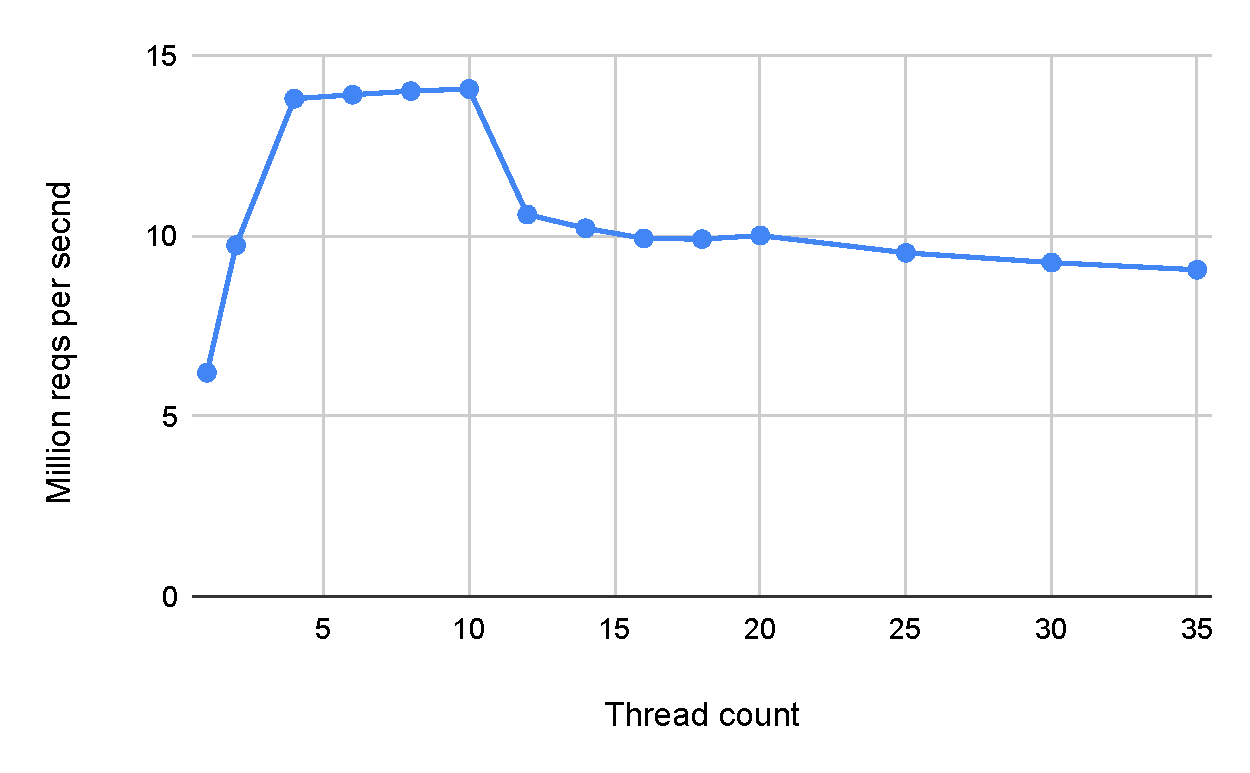
\includegraphics[width=\textwidth]{1_figures/ZAB-scal.pdf}
%     % \captionsetup{width=0.85\linewidth}
%     % \vspace{-1.8em}
%   \caption{Write-only throughput of ZAB and MP, varying the workers}
% %   \vspace{-1.5em}
%   \label{fig:zab-scal}
%   \end{subfigure} %%
  
% \begin{subfigure}[b]{0.33\textwidth}
% 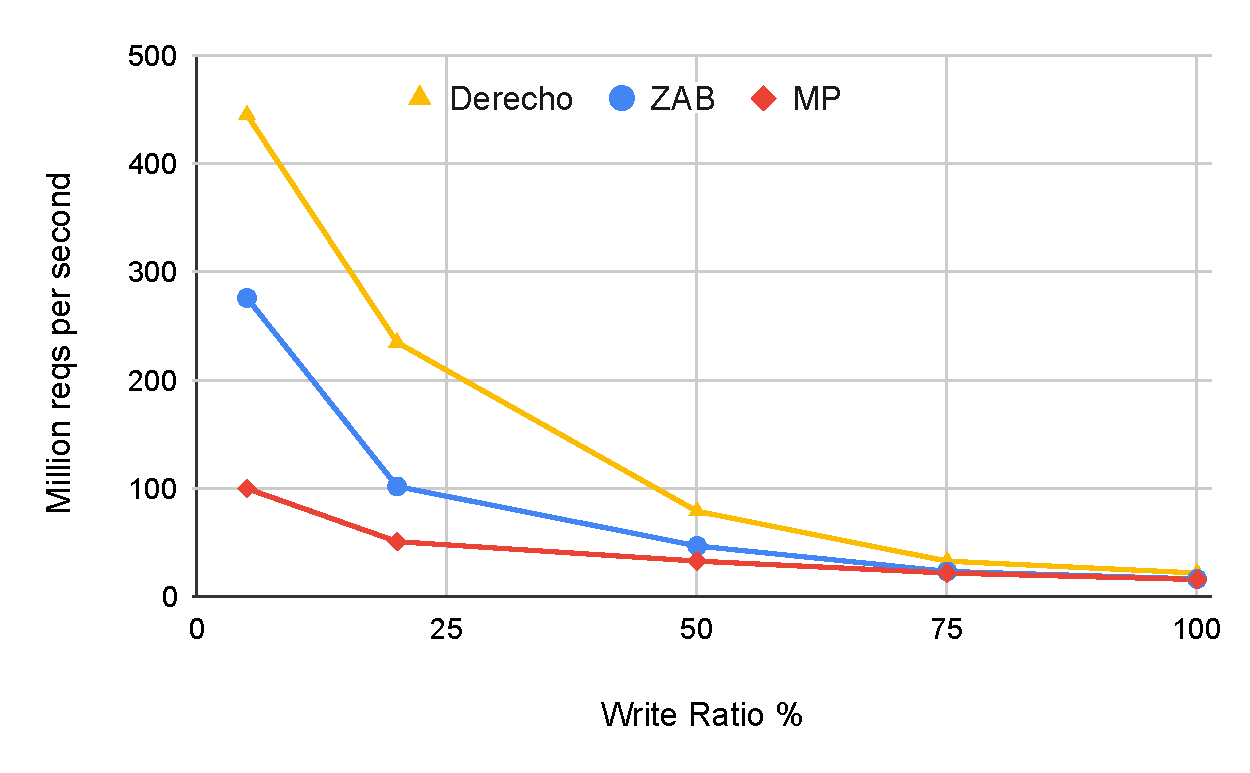
\includegraphics[width=\textwidth]{1_figures/zab-mp-dr.pdf}
% % \captionsetup{width=0.85\linewidth}
% % \vspace{-1.8em}
% \caption{Throughput of ZAB, MP \& Derecho, varying the write ratio from 1\% to 100\%}
% %   \vspace{-1.5em}
% \label{fig:zab-mp-dr}
% \end{subfigure}%

% \begin{subfigure}[b]{0.33\textwidth} 

% 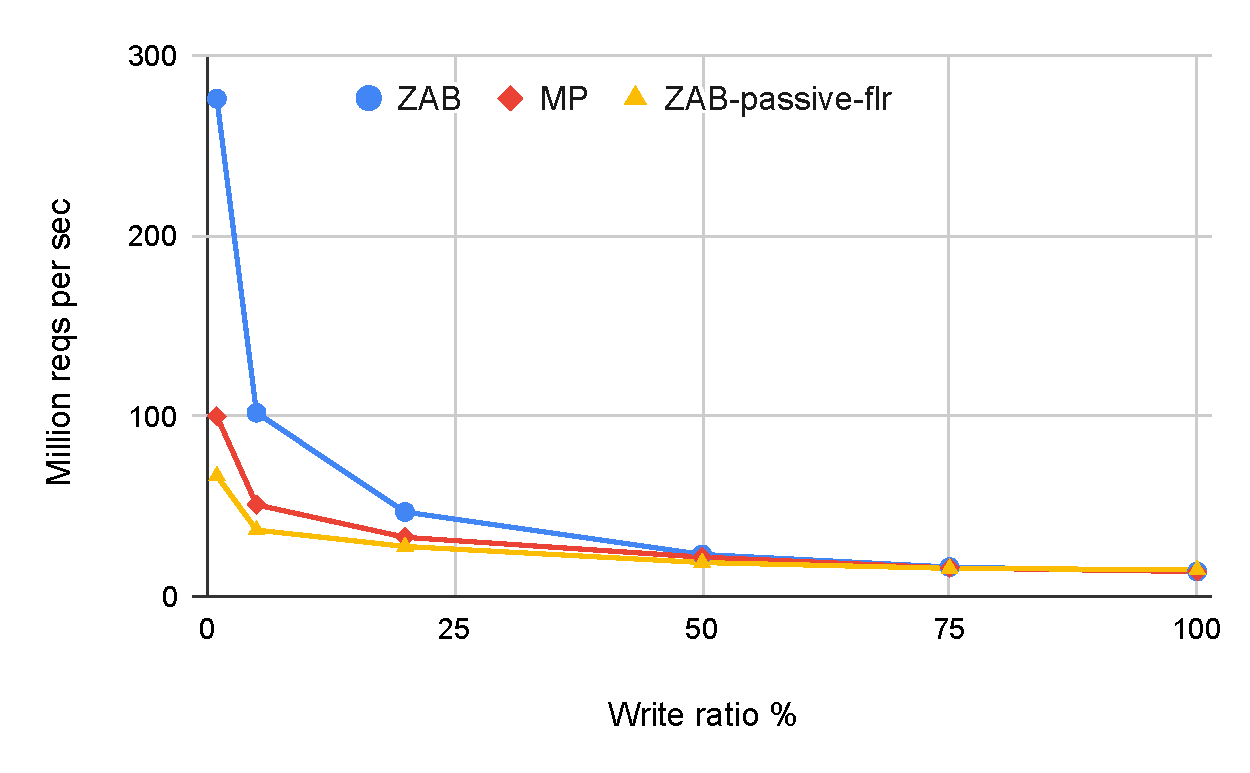
\includegraphics[width=\textwidth]{1_figures/zab-passive-flr.pdf}
% %   \vspace{-0.5em}
% \caption{Throughput of ZAB, MP and ZAB/MP with passive followers, when varying the write ratio}
% %   \vspace{-1.5em}
% \label{fig:zab-psv}
% \end{subfigure}%
% %   \vspace{-2em}
% \caption{\LTO~graphs. }
% \label{fig:lto}
% %   \vspace{-1.5em}
% \end{figure*}
\begin{table}[t]
\centering
 \resizebox{0.48\textwidth}{!}{%
\begin{tabular}{c|c|c|c|c|c|c|c|||c|c|c|c|c|}
\hhline{~-----------}
& \multicolumn{7}{c|||}{\colorhl\textbf{ Throughput vs. Write ratio}} &
\multicolumn{4}{c|}{\colorhl\textbf{ Latency vs. Load}}
 \\ 
 \hhline{~-----------}


\textbf{}                                                               
& 
 \colorhl%
{0\%} &
 \colorhl%
{1\%} &
 \colorhl%
{5\%} &
 \colorhl%
{20\%}&
 \colorhl%
{50\%}&
 \colorhl%
{75\%}&
 \colorhl%
{100\%} & 

 \colorhl%
{25\%} &
 \colorhl%
{50\%} &
 \colorhl%
{75\%} &
 \colorhl%
{100\%}
\\  
\hhline{~-----------}
\hline




\multicolumn{1}{|c|}{\colorhl ZAB} &
967 &	276 &	102 &	47 &	23.5 &	16.5 &	14 
& 
22 / 16 & 
30 / 23 & 
40 / 32 & 
110 / 95
 \\ \hline \hline
 \greyrow
\multicolumn{1}{|c|}{\colorhl MP} &
170 &	100 &	51 &	33 &	22 &	16 &	14 
&
22 / 16 & 
30 / 23 & 
40 / 32 & 
110 / 95
 \\ \hline \hline
\multicolumn{1}{|c|}{\colorhl Derecho} &
967 &	445 &	235 &	79 &	33 &	22 &	16.6 
&
16 / 13 & 
24 / 19 & 
32 / 27 & 
94 / 86
 \\ \hline \hline
 \greyrow
  \multicolumn{1}{|c|}{\colorhl CP} &
125 &	115 &	90 &	65 &	44 &	35 &	27 
&
38 / 26 & 
40 / 33 & 
56 / 47 & 
216 / 163
 \\ \hline \hline
\multicolumn{1}{|c|}{\colorhl CHT} &
967 &	755 &	520 &	134 &	53 &	36 &	28 
&16 / 16 & 
24 / 19 & 
38 / 31 & 
282 / 209
 \\ \hline \hline
 \greyrow
\multicolumn{1}{|c|}{\colorhl All-Aboard} &
125 &	116 &	92 &	70 &	51 &	42 &	39 
&
24 / 18 & 
38 / 27 & 
58 / 40 & 
252 / 167
 \\ \hline \hline
\multicolumn{1}{|c|}{\colorhl ABD} &
125 &	118 &	102 &	84 &	71 &	64 &	61 
&
28 / 26 & 
34 / 33 & 
52 / 47 & 
138 / 163
 \\ \hline \hline
 \greyrow
 \multicolumn{1}{|c|}{\colorhl CRAQ} &
967 &	739 &	476 &	246 &	123 &	87 &	67 
&
34 / 22 & 
48 / 30 & 
58 / 37 & 
242 / 138
 \\ \hline \hline
\multicolumn{1}{|c|}{\colorhl CHT-multi-ldr} &
967 &	674 &	443 &	192 &	134 &	97 &	76
&30 / 19 & 
82 / 58 & 
86 / 59 & 
554 / 323

 \\ \hline \hline
 \greyrow
\multicolumn{1}{|c|}{\colorhl CHT-mcast} &
967 &	745 &	524 &	277 &	145 &	105 &	85 
&
20 / 14 & 
24 / 16 & 
40 / 26 & 
210 / 147
 \\ \hline \hline

\multicolumn{1}{|c|}{\colorhl Hermes} &
967 &	735 &	515 &	275 &	150 &	107 &	89 
& 18 / 13 & 
24 / 15 & 
36 / 22 & 
110 / 78 
 \\ \hline 


\end{tabular}%
 }
\caption{Left-hand side: Throughput in M.reqs/s varying the write ratio. Right-hand side: 99th percentile and average latency (99th/ avg) in $\mu$seconds varying the load in a write-only workload.}
\vspace{-1.5em}
\label{tab:all-perf}
\end{table}

















% \begin{table}[t]
\centering
% \footnotesize
 \resizebox{0.38\textwidth}{!}{%
\begin{tabular}{c|c|c|c|c|c|c|c|}
% \hline
\hhline{~-------}
\textbf{}                                                               
%\begin{tabular}[c]{@{}c@{}}write\\ ratio \end{tabular}
& 
 \colorhl\textbf
{0\%} &
 \colorhl\textbf
{1\%} &
 \colorhl\textbf
{5\%} &
 \colorhl\textbf
{20\%}&
 \colorhl\textbf
{50\%}&
 \colorhl\textbf
{75\%}&
 \colorhl\textbf
{100\%}
\\  \hline
%%%%%%%%%%

\multicolumn{1}{|c|}{\colorhl ZAB} &
967 &	276 &	102 &	47 &	23.5 &	16.5 &	14 
 \\ \hline \hline
 %%%%%%%%%%
 \greyrow
\multicolumn{1}{|c|}{\colorhl MP} &
170 &	100 &	51 &	33 &	22 &	16 &	14 
 \\ \hline \hline
 %%%%%%%%%%
\multicolumn{1}{|c|}{\colorhl Derecho} &
967 &	445 &	235 &	79 &	33 &	22 &	16.6 
 \\ \hline \hline
 %%%%%%%%%%
 \greyrow
  \multicolumn{1}{|c|}{\colorhl CP} &
125 &	115 &	90 &	65 &	44 &	35 &	27 
 \\ \hline \hline
 %%%%%%%%%%
\multicolumn{1}{|c|}{\colorhl CHT} &
967 &	755 &	520 &	134 &	53 &	36 &	28 
 \\ \hline \hline
  %%%%%%%%%%
 \greyrow
\multicolumn{1}{|c|}{\colorhl All-Aboard} &
125 &	116 &	92 &	70 &	51 &	42 &	39 
 \\ \hline \hline
 %%%%%%%%%%
\multicolumn{1}{|c|}{\colorhl ABD} &
125 &	118 &	102 &	84 &	71 &	64 &	61 
 \\ \hline \hline
 %%%%%%%%%%
 \greyrow
 \multicolumn{1}{|c|}{\colorhl CRAQ} &
967 &	739 &	476 &	246 &	123 &	87 &	67 
 \\ \hline \hline
 %%%%%%%%%%
\multicolumn{1}{|c|}{\colorhl CHT-multi-ldr} &
967 &	674 &	443 &	192 &	134 &	97 &	76
 \\ \hline \hline
 %%%%%%%%%%
 \greyrow
\multicolumn{1}{|c|}{\colorhl CHT-mcast} &
967 &	745 &	524 &	277 &	145 &	105 &	85 
 \\ \hline \hline
 %%%%%%%%%%

\multicolumn{1}{|c|}{\colorhl Hermes} &
967 &	735 &	515 &	275 &	150 &	107 &	89 
 \\ \hline 
 %%%%%%%%%%



% \multicolumn{1}{|c|}{
% \colorhl ZAB} & 
% 967 &  276  & 102  &47  &23.5  &16.5  &14  
%  \\ \hline
% %%%%%%%%%%
% \multicolumn{1}{|c|}{
% \colorhl MP} & 
% 170 &  100  & 51  & 33  & 22  & 16  & 14  
%  \\ \hline
% %%%%%%%%%%
% \multicolumn{1}{|c|}{\colorhl Derecho} &
% 16.6	&22.15	&33.35	&79	&235	&445	&967
% \\ \hline
% %%%%%%%%%%%%%%%%%
% \multicolumn{1}{|c|}{\colorhl CP} &
% 25	&35	&44	&65	&90	&115	&125
% \\ \hline
% %%%%%%%%%%%%%%%%%
% \multicolumn{1}{|c|}{\colorhl CHT} &
% 27	&36	&53	&134	&520	&755	&967
% \\ \hline
% %%%%%%%%%%%%%%%%%
% \multicolumn{1}{|c|}{\colorhl All-Aboard} &
% 38	&42	&51	&70	&92	&116	&125
% \\ \hline
% %%%%%%%%%%%%%%%%%
% \multicolumn{1}{|c|}{\colorhl ABD} &
% 61	&64	&71	&84	&102	&118	&125
% \\ \hline
% %%%%%%%%%%%%%%%%%
% \multicolumn{1}{|c|}{\colorhl CHT-multi-ldr} &
% 66	&97	&134	&192	&443	&674	&967
% \\ \hline
% %%%%%%%%%%%%%%%%%
% \multicolumn{1}{|c|}{\colorhl CRAQ} &
% 67	&87	&123	&246	&476	&739	&967
% \\ \hline
% %%%%%%%%%%%%%%%%%
% \multicolumn{1}{|c|}{\colorhl CHT-mcast} &
% 80	&105	&145	&277	&524	&745	&967
% \\ \hline
% %%%%%%%%%%%%%%%%%
% \multicolumn{1}{|c|}{\colorhl Hermes} &
% 89	&107	&150	&275	&515	&735	&967
% \\ \hline
% %%%%%%%%%%%%%%%%%



\end{tabular}%
 }
\caption{Throughput in M.reqs/s varying the write ratio}
\label{tab:all-perf}
\end{table}
% \begin{table}[t]
\centering
% \footnotesize
 \resizebox{0.38\textwidth}{!}{%
\begin{tabular}{c|c|c|c|c|}
% \hline
\hhline{~----}
\textbf{}                                                               
%\begin{tabular}[c]{@{}c@{}}write\\ ratio \end{tabular}
& 
 \colorhl\textbf
{25\%} &
 \colorhl\textbf
{50\%} &
 \colorhl\textbf
{75\%} &
 \colorhl\textbf
{100\%}
\\  \hline
%%%%%%%%%%

\multicolumn{1}{|c|}{\colorhl ZAB} &
22 / 16 & 
30 / 23 & 
40 / 32 & 
110 / 95
 \\ \hline \hline
 %%%%%%%%%%
 \greyrow
\multicolumn{1}{|c|}{\colorhl MP} &
22 / 16 & 
30 / 23 & 
40 / 32 & 
110 / 95
 \\ \hline \hline
 %%%%%%%%%%
\multicolumn{1}{|c|}{\colorhl Derecho} &
16 / 13 & 
24 / 19 & 
32 / 27 & 
94 / 86
 \\ \hline \hline
 %%%%%%%%%%
 \greyrow
  \multicolumn{1}{|c|}{\colorhl CP} &
38 / 26 & 
40 / 33 & 
56 / 47 & 
216 / 163
 \\ \hline \hline
 %%%%%%%%%%
\multicolumn{1}{|c|}{\colorhl CHT} &
16 / 16 & 
24 / 19 & 
38 / 31 & 
282 / 209
 \\ \hline \hline
  %%%%%%%%%%
 \greyrow
\multicolumn{1}{|c|}{\colorhl All-Aboard} &
24 / 18 & 
38 / 27 & 
58 / 40 & 
252 / 167
 \\ \hline \hline
 %%%%%%%%%%
\multicolumn{1}{|c|}{\colorhl ABD} &
28 / 26 & 
34 / 33 & 
52 / 47 & 
138 / 163
 \\ \hline \hline
 %%%%%%%%%%
 \greyrow
 \multicolumn{1}{|c|}{\colorhl CRAQ} &
34 / 22 & 
48 / 30 & 
58 / 37 & 
242 / 138
 \\ \hline \hline
 %%%%%%%%%%
\multicolumn{1}{|c|}{\colorhl CHT-multi-ldr} &
30 / 19 & 
82 / 58 & 
86 / 59 & 
554 / 323
 \\ \hline \hline
 %%%%%%%%%%
 \greyrow
\multicolumn{1}{|c|}{\colorhl CHT-mcast} &
20 / 14 & 
24 / 16 & 
40 / 26 & 
210 / 147
 \\ \hline \hline
 %%%%%%%%%%

\multicolumn{1}{|c|}{\colorhl Hermes} &
18 / 13 & 
24 / 15 & 
36 / 22 & 
110 / 78 
 \\ \hline 
 %%%%%%%%%%
\end{tabular}%
 }
\caption{99th percentile and average latency (99the/ avg) in useconds for 25\% 50\%, 75\% and 100\% load in a write-only workload.}
\label{tab:all-lat}
\end{table}




\subsection{\LTO: ZAB and Multi-Paxos}\label{sec:ev:lto}


In this section, we first briefly describe the operation of our two implemented \LTO~protocols: ZAB and Multi-Paxos (MP). 
Then we focus on their results, first discussing thread-scalability for write throughput, and then the throughput when varying the write ratio.
% Notably, our ZAB and MP significantly outperform their open-source counterparts whose throughput are a few thousand requests per second. (ZAB as evaluated in ~\cite{Jin:2018} and MP as evaluated in~\cite{Liu:2020}).



\beginbsec{ZAB \& MP operation}
All writes must be propagated to the leader which executes them in two broadcast rounds: a prepare round and a commit round.
The difference between ZAB and MP is in reads. ZAB executes reads locally downgrading consistency guarantees to SC.
MP offers lin, and so, all reads are sent to the leader.


\begin{comment}
Let's go through an example of the operation.
As in all \odlib~protocols, each node contains a number of worker threads.
% The leader node and the follower nodes execute different code.
Assume worker-0 of the leader pulls 100 writes from the clients.
Each write must be allocated a slot (write-id) in the total order. To achieve that, the worker fetches a global counter, that contains the highest write-id that has been allocated, and increments it by 100 (with an atomic fetch-and-add). Assume the counter was initially 200 and was modified to 300.
The worker tags each write with a unique write-id ranging from 200 to 300, and then broadcasts them all to the worker-0 of all followers. Each follower's worker-0 buffers the write and responds with a smart-ack (one ack for all 100 writes, described in \secref{sec:nw:sm}). Upon receiving a majority of the acks, leader's worker-0 broadcasts a smart-com (one commit for all 100 writes, also described in \secref{sec:nw:sm}).

\custvspace
Reads in ZAB are executed locally. Upon pulling a batch of reads, the worker propagates them to the KVS layer which directly responds to the client.
In MP, all reads must be sent to leader, to ensure linearizability.
Similarly to acks and commits, reads are also smart. The KVS stores a version number along with each key. The version number is updated on each write with the unique write-id.
A read request from a follower to the leader contains the key and the locally stored version. The leader replies with the value iff its stores a later version than the follower. Otherwise, it replies with a simple 1-byte opcode notifying the follower that its version is up to date.
\end{comment}


\beginbsec{Thread-scalability}
The thread-scalability problem occurs when the different workers, either in the leader or the followers, try to apply the writes to the KVS. For example, the write with write-id = 200 (\ie write-200), can only be applied \emph{after} write-199 has been applied. If worker-0 is responsible for applying write-200, but not write-199, then 
worker-0 must wait until the worker responsible for write-199 applies it.
Therefore the thread-scalability problem rises from the fact that workers can only apply their writes to the KVS in lock-step. \figref{fig:zab-scal} shows the write-only throughput of ZAB and MP when varying the number of threads (\ie workers). 
Scaling saturates at four workers.
% The design scales well until four workers and then saturates.
When deployed with more than 10 workers, the performance drops because the additional workers are pinned to the second socket of the server, hindering inter-thread communication.




\beginbsec{Throughput when varying the write ratio}
% \tabref{tab:all-perf} lists the throughput of ZAB and MP when varying the write ratio. 
\figref{fig:zab-mp-dr} compares the throughput of ZAB and MP with Derecho, when varying the write ratio.
%comparing with the protocol's closest neighbour, Derecho.
ZAB's consistency relaxation that allows for local reads pays off, as ZAB significantly outperforms MP in low write ratios. 

However, note that ZAB's write throughput does not scale well in low write ratios. For instance, at 5\% write ratio, ZAB achieves 102 M.reqs/s, which means that its write throughput is roughly 5 million per sec. Ideally, since local reads are fairly cheap, one might expect that ZAB should have been able to maintain its peak write throughput (14m at 100\% write ratio) at lower write ratios. Note that Derecho maintains its 16.6m write throughput at both 75\% write ratio and 50\% write ratio. Derecho is able to sustain its write throughput better due to its decentralized nature and thus outperforms ZAB in lower write ratios. In contrast, in ZAB (and MP), followers must send their writes to the leader which coordinates their execution. When decreasing the write ratio, the ability to batch multiple writes together into network packets and steer them into the leader is disrupted by the execution of reads, and so the write throughput cannot be maintained.



\beginbsec{Passive followers}
In order to examine whether it would be beneficial to spawn requests only at the leader node, \figref{fig:zab-psv} shows the throughput of \emph{ZAB-passive-flr}, a ZAB variant where followers are passive: \ie followers are not connected with clients and thus do not initiate the execution of requests. Rather, only the leader initiates requests, while followers are only used to help coordinate writes. 
In this case, MP and ZAB are identical, because in both protocols reads at the leader can execute locally.
ZAB-passive-flr can achieve the same write throughput as ZAB at 100\% write ratio because all writes must execute at the leader anyway. However, its performance degrades as reads increase. The reason is that the single node (\ie the leader) cannot compete with a 5-node deployment when it comes to executing local reads. Specifically, followers' cpu and memory resources must be utilized to scale at low write ratios. Therefore active followers that are responsible for client sessions are beneficial. This result holds for \LPKO~protocols, too.

\begin{comment}
\beginbsec{Summary}
In this section, we  have made the following observations. Firstly, total order hinders thread-scalability. 
Secondly, a low write throughput can prevent local reads from providing good performance even at low-write ratios.
Finally, we saw that passive followers are detrimental for performance.
Notably, these generic results hold for all classes.
\end{comment}
% \begin{figure}[t]
  \centering
  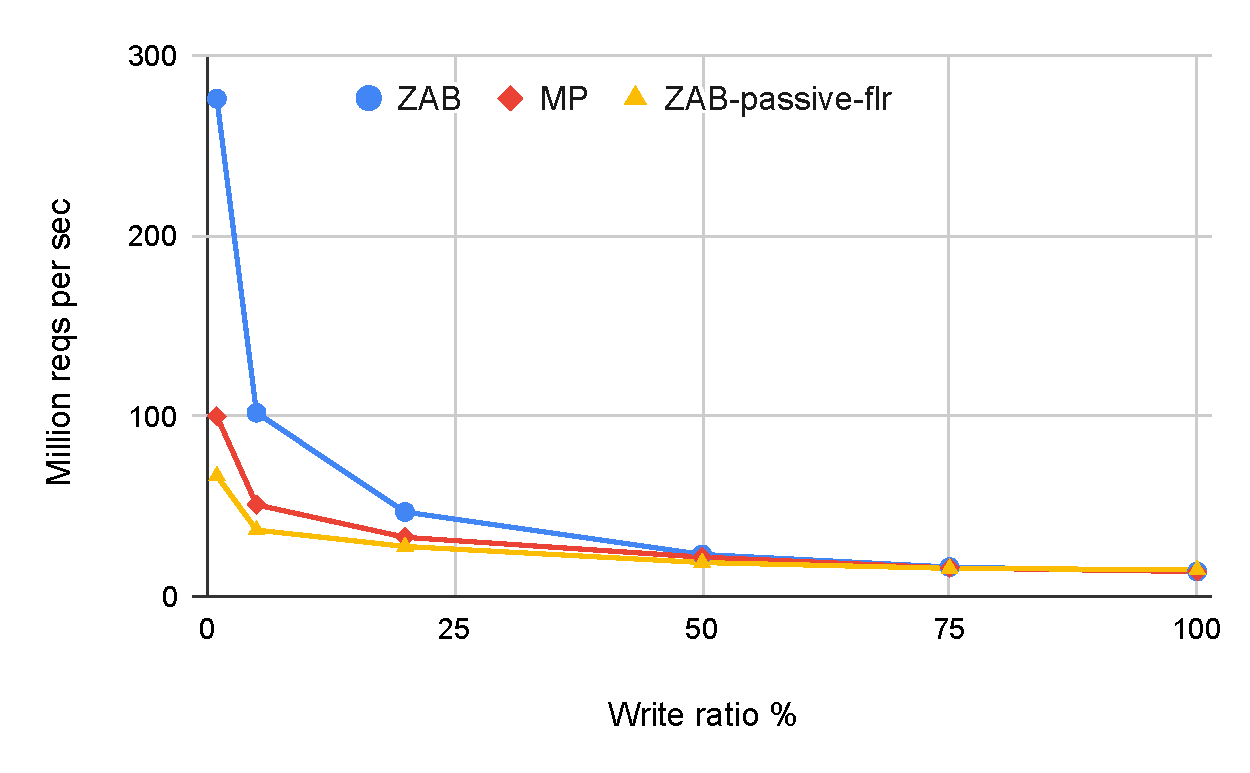
\includegraphics[scale=0.4]{1_figures/zab-passive-flr.pdf}
%   \vspace{-0.5em}
  \caption{Throughput of ZAB, MP and ZAB/MP with passive followers, when varying the write ratio}
%   \vspace{-1.5em}
  \label{fig:zab-psv}
\end{figure}
% \begin{figure}[t]
  \centering
  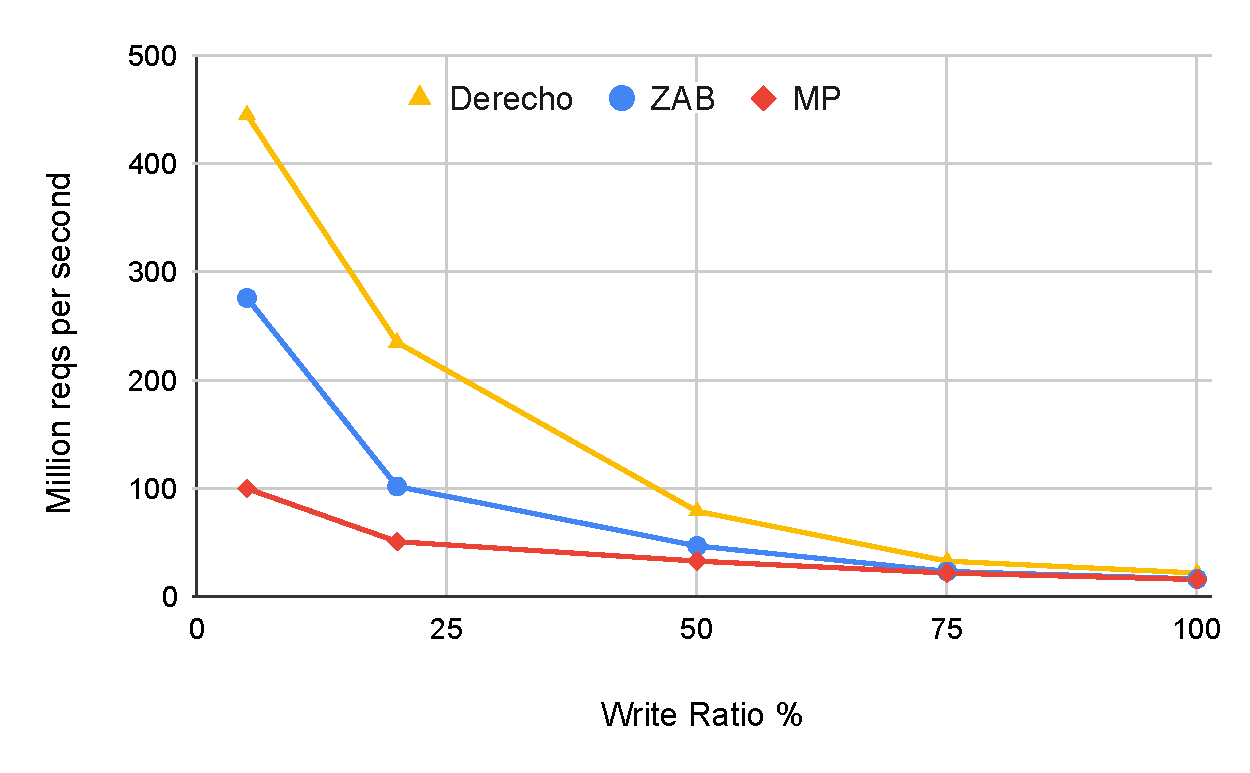
\includegraphics[scale=0.4]{1_figures/zab-mp-dr.pdf}
%   \vspace{-0.5em}
  \caption{Throughput of ZAB, MP \& Derecho, varying the write ratio from 1\% to 100\%}
%   \vspace{-1.5em}
  \label{fig:zab-mp-dr}
\end{figure}
% \begin{figure}[t]
  \centering
  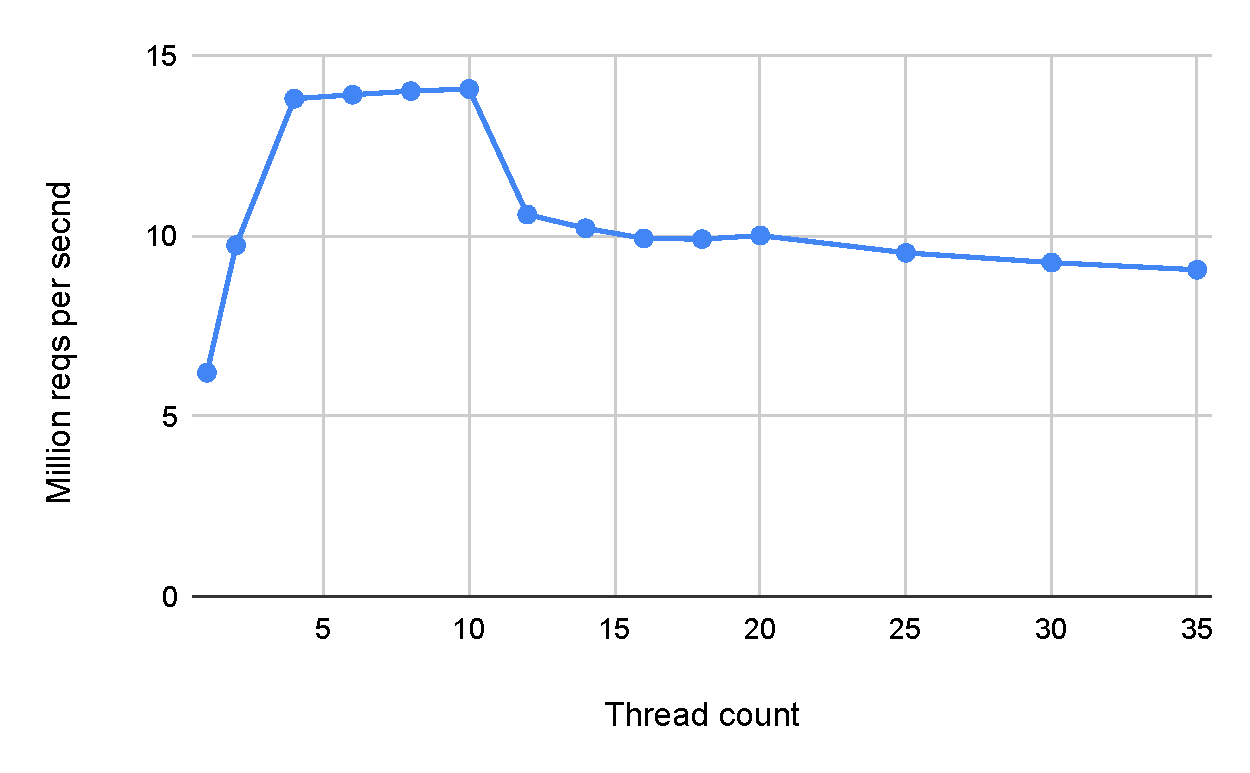
\includegraphics[scale=0.4]{1_figures/ZAB-scal.pdf}
%   \vspace{-0.5em}
  \caption{Write-only throughput of ZAB and MP, varying the workers [5 nodes]}
%   \vspace{-1.5em}
  \label{fig:zab-scal}
\end{figure}
% \begin{figure}[t]
  \centering
  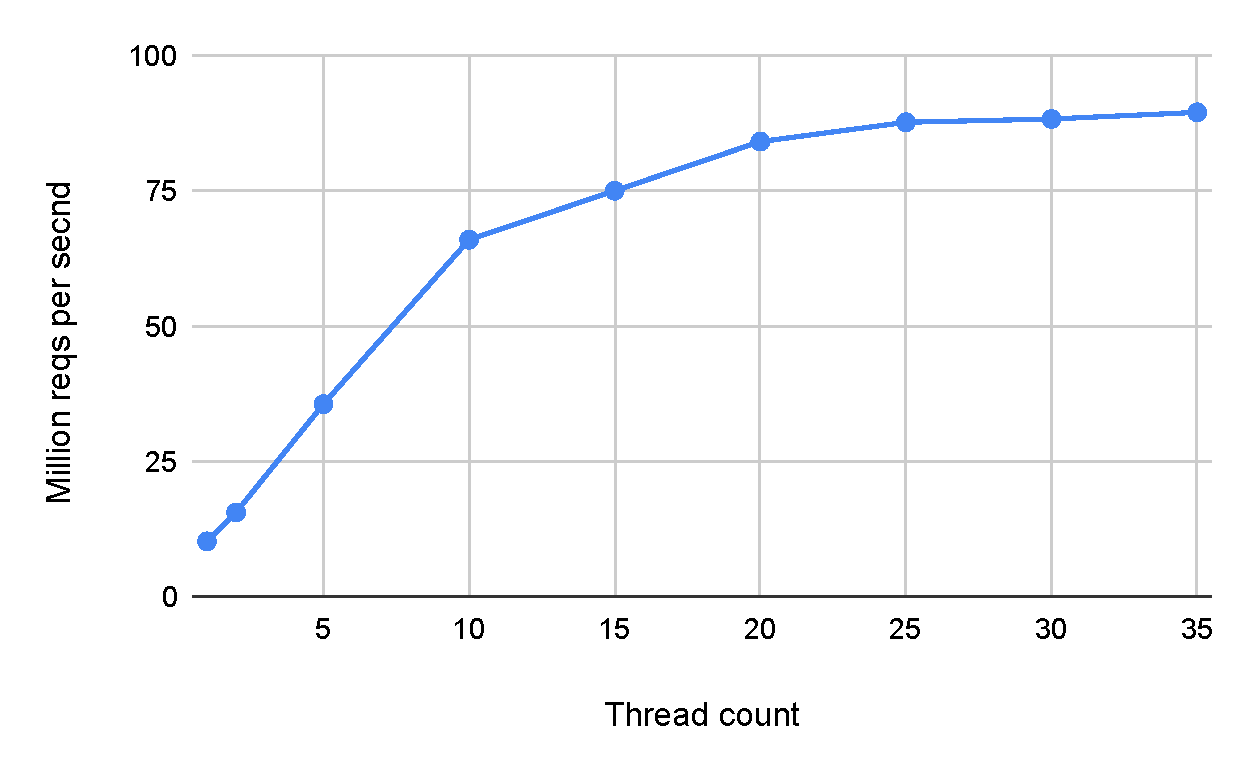
\includegraphics[scale=0.4]{1_figures/Hr-scal.pdf}
%   \vspace{-0.5em}
  \caption{Write-only throughput of Hermes, varying the workers [5 nodes]}
%   \vspace{-1.5em}
  \label{fig:hr-scal}
\end{figure}



\subsection{\DTO: Derecho}\label{sec:ev:dto}
We have already established the effects of the total order in write throughput and contrasted Derecho with ZAB and MP. 
Here we will briefly describe Derecho's operation and comment on its performance in lower write ratios, contrasting it with two \DPKO~protocols.
% Notably our Derecho significantly outperforms the open-source system which performs roughly 250k reqs per second (as evaluated in~\cite{A:2020}) \antonis{Consider downplaying a bit -- e.g., Dereco is a fuller-system(?)}.



\beginbsec{Derecho operation}
In Derecho, writes are totally ordered and applied in that order. The different write-ids are statically pre-allocated to different nodes. Node-0 will propose writes $0$ to $N-1$, node-1 will propose writes $N$ to $2N - 1$, and so on.
Furthermore, Derecho performs reads locally, relaxing the consistency guarantees from lin to SC (similarly to ZAB). 

\begin{comment}
Let us now briefly discuss how we have implemented Derecho.
For each machine we pre-allocate a number of write-ids, in a round-robin fashion. A node's pre-allocated write-ids are again pre-allocated to the workers within it. Therefore, a worker need not synchronize with other workers to discover the next write-id it must use; rather it computes it from its own worker-id and node-id.
Similarly to ZAB, a write requires two broadcast rounds, a prepare and a commit. The receiver of a prepare responds with an ack (implemented with \odlib~ smart-acks). The receiver of a commit, which is also implemented with \odlib~smart-com, need not reply.
Finally, reads are implemented identically to ZAB.
\end{comment}
% \beginbsec{Reads}
\beginbsec{Performance}
Without considering thread-scalability, \DTO\ is a powerful idea as the different nodes need not coordinate in order to serialize the writes. They merely need to compute the order of their own writes through their node-id and broadcast them.
This is why 
Derecho is one of the better performing protocols in single-threaded performance (\figref{fig:single-thr}). 
However, as we saw with ZAB and MP, applying writes in a total order does not scale across many threads.

As discussed in the previous section, Derecho scales better than ZAB at lower write ratios (\figref{fig:zab-mp-dr}); however its low write throughput still limits its total throughput at low write ratios.
%is still limited by its small write throughput.
For instance, when compared with Hermes (lin local reads) and CP (ABD reads) in \figref{fig:hr-dr-cp}, Derecho is significantly outperformed by Hermes even in low write ratios, because Hermes has a higher write throughput (due to its thread-scalability), which allows it to scale well at low write ratios. 
% In contrast, the low write throughput of Derecho, limits its throughput
However, Derecho's local reads allow it to outperform CP, on low write ratios, despite the fact that CP has a higher write throughput.

\begin{figure*}[t]
\centering
  \begin{subfigure}[t]{0.33\textwidth}
    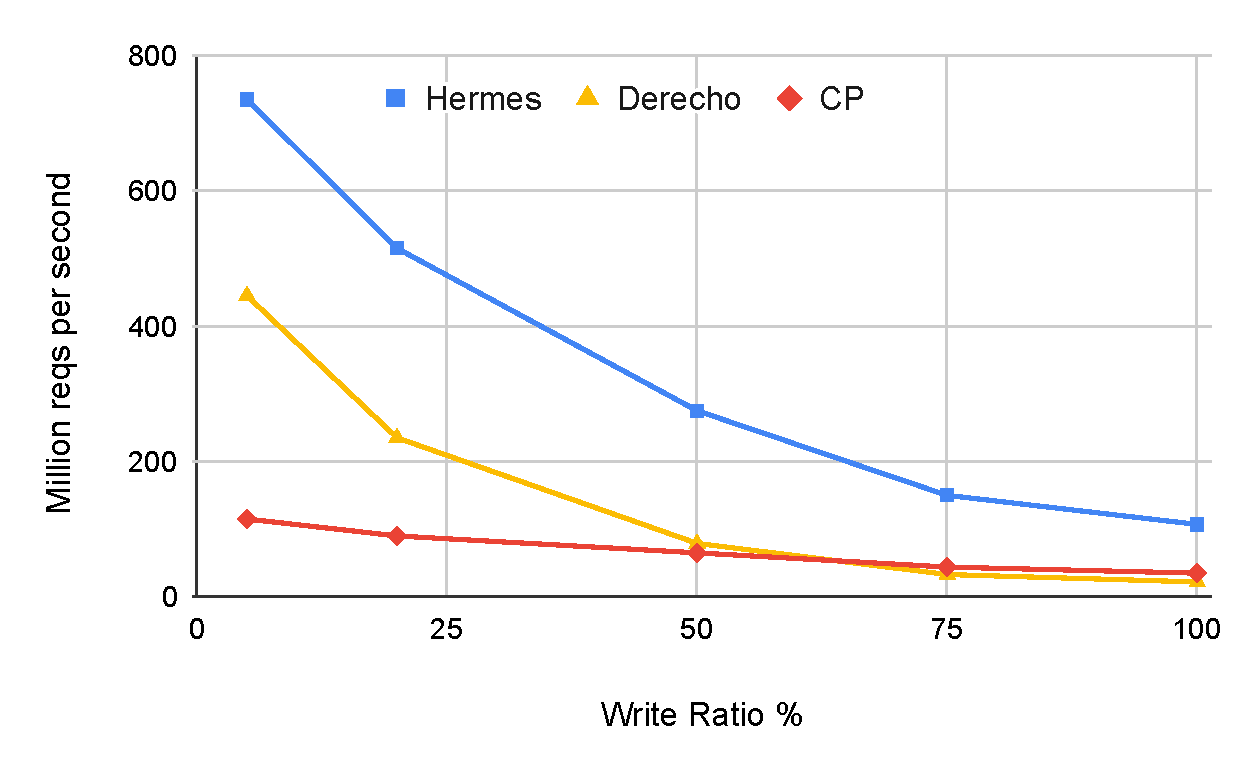
\includegraphics[width=\textwidth]{1_figures/hr-dr-cp.pdf}
    \captionsetup{width=\linewidth}
    % \vspace{-1.8em}
   \caption{Hermes, Derecho \& CP}
%   \vspace{-1.5em}
  \label{fig:hr-dr-cp}
  \end{subfigure}
  %
  \begin{subfigure}[t]{0.33\textwidth}
    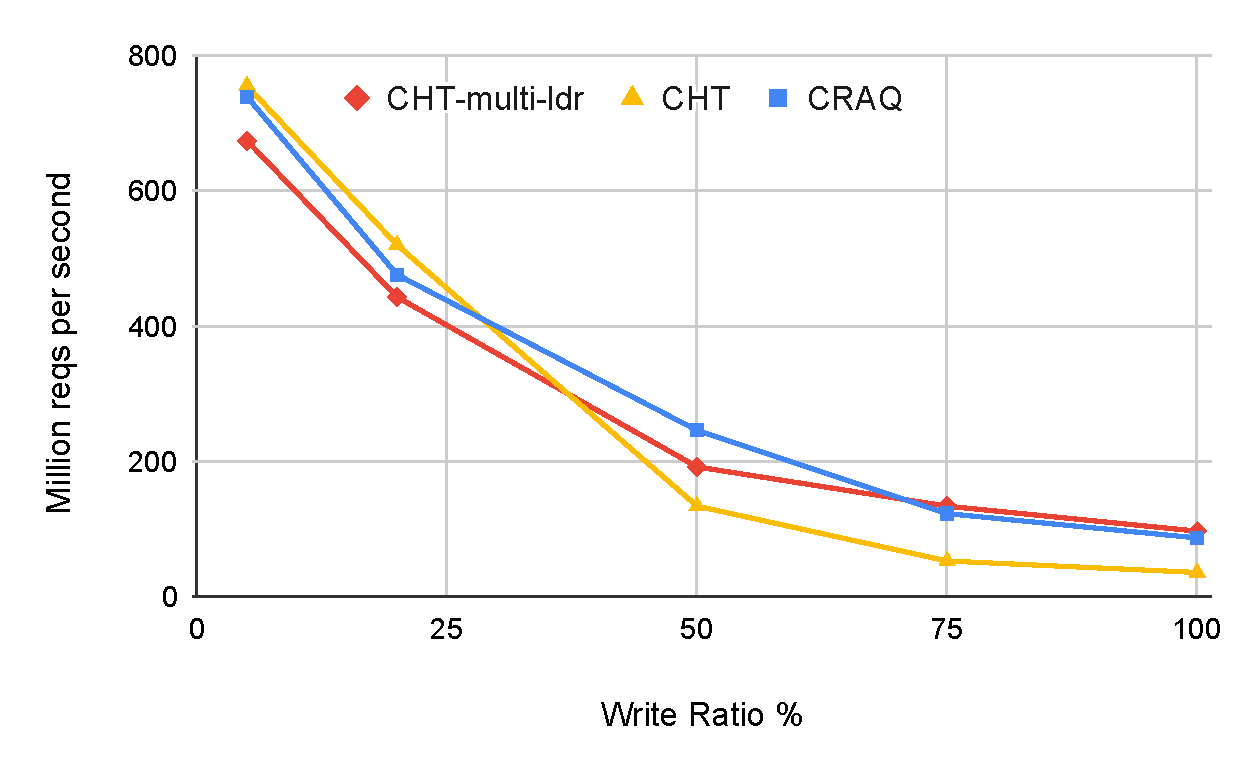
\includegraphics[width=\textwidth]{1_figures/craq-cht-chtml.pdf}
    \captionsetup{width=0.95\linewidth}
    % \vspace{-1.8em}
    \caption{CHT-multi-ldr, CHT \& CRAQ}
%   \vspace{-1.5em}
  \label{fig:cht-cht-craq}
  \end{subfigure}
  %
  \begin{subfigure}[t]{0.33\textwidth} 
  
    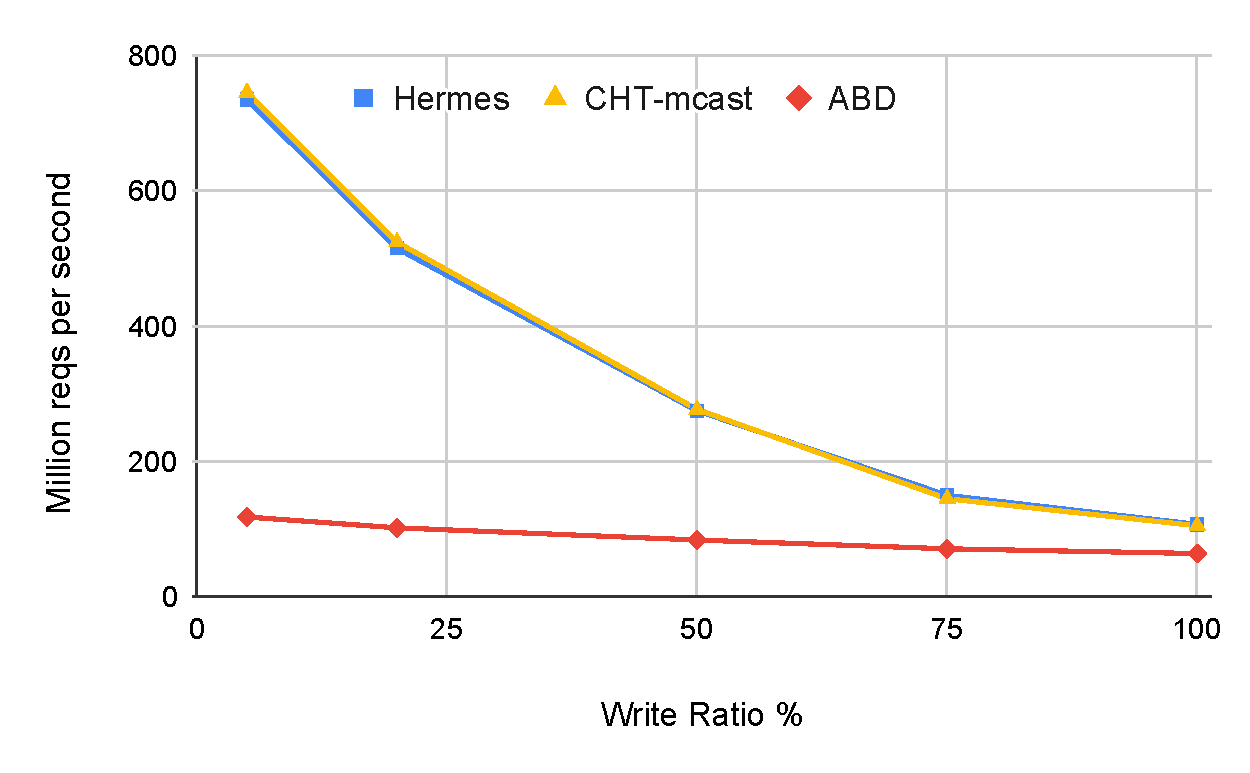
\includegraphics[width=\textwidth]{1_figures/hr-chtm-abd.pdf}
    \captionsetup{width=0.90\linewidth}
    % \vspace{-1.8em}
    \caption{Hermes, CHT-mcast \& ABD}
%   \vspace{-1.5em}
  \label{fig:hr-cht-abd}
  \end{subfigure}
%   \vspace{-1em}
  \caption{Throughput vs. write ratio}
  \label{fig:three-graphs}
%   \vspace{-1em}
\end{figure*}

% \begin{figure}[t]
%   \centering
%   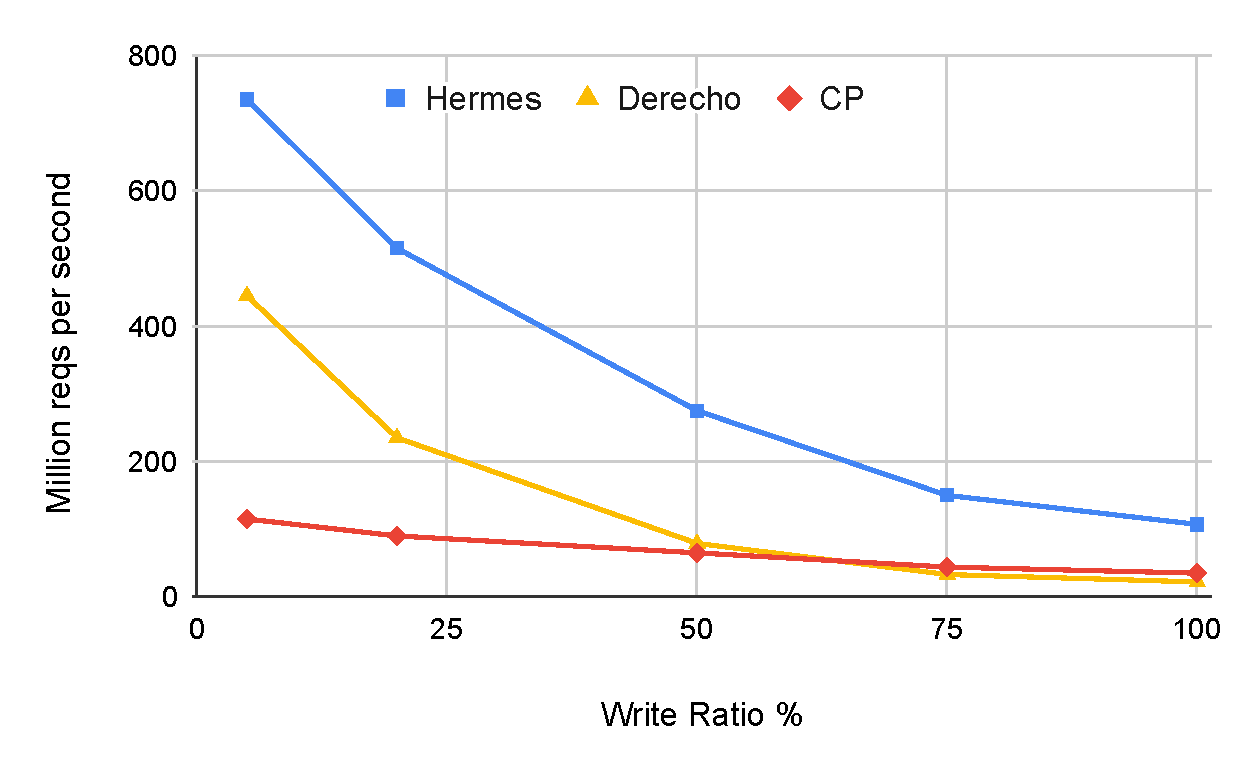
\includegraphics[scale=0.4]{1_figures/hr-dr-cp.pdf}
% %   \vspace{-0.5em}
%   \caption{Throughput of Hermes, Derecho \& CP, varying the write ratio from 1\% to 100\%}
% %   \vspace{-1.5em}
%   \label{fig:hr-dr-cp}
% \end{figure}

\subsection{\LPKO: CHT, CHT-multi-ldr, and CRAQ}\label{sec:ev:lpko}

We start the discussion of the \LPKO~protocols with CHT and then extend it to CRAQ. 

% To the best of our knowledge this is the first implementation of CHT. CHT-multi-ldr is similar to FGSMR~\cite{Liu:2020}, whose performance is significantly lower at a few hundred thousand requests per second. Finally, the throughput of the CRAQ open-source implementation~\cite{Terrace:2009} is a few thousand requests per second.

\beginbsec{CHT operation}
All writes in CHT are propagated to the leader. The leader completes the writes in two broadcast rounds, similarly to ZAB and MP, with two differences: 1) it does not create a total order of all writes and 2) it waits until a write has reached all followers before committing it. 
The latter allows for local reads at the follower nodes. Notably, reads need to block if there is an ongoing write to the same key, until that write commits. %; when the write commits the read can complete. %This blocking is inevitable for lin reads, as proven in the CHT paper~\cite{Chandra:2016}

\begin{comment}
Let us briefly discuss a few implementation details.
Firstly note that reads are subtly different than ZAB and Derecho.
Specifically, because reads are lin, it must be that once a read returns a value, a later read can never return an earlier value. To achieve this, we maintain a state variable with each key, initially denoting that the key is \qt{valid} and can be read. Upon receiving the first round of a write, the state transitions to \qt{invalid}, denoting that the value cannot be read until the write is committed. Reads that find a key in invalid state will be buffered to be retried in the future. Note that this blocking of lin reads is inevitable as proven in the CHT paper~\cite{Chandra:2016}. 

The implementation of writes are again similar to ZAB and MP with a subtle difference.
In order to support multi-threading, we have added a version to each key (as part of its metadata).
The per-key version is incremented by the leader, each time it writes the key. Then the version is sent along with the write in the first broadcast round.
To understand why the version is necessary assume that two different workers of the leader attempt to write the same key concurrently. 
The two writes will serialize at he leader node due to the concurrency control at the KVS: whoever grabs the lock first will also write first.
However, that ordering of the two writes must be honoured in the follower nodes. This will be achieved with the per-key version. Plainly, the version of the later write will be bigger, allowing the followers to serialize the writes in the correct order.
\end{comment}

In CHT-multi-ldr each node is the leader for $1/N$ of all keys, with $N$ being the number of nodes. 
% The partitioning is done by using modulo N on the key.
% Therefore, u
Upon receiving a write request for key $K$, the worker finds out the leader for that key through a simple modulo operation on the key. Then, similarly to CHT, the write is propagated to its leader, which executes it to completion. %In our setup this simple partitioning scheme creates a uniform distribution of keys to leaders.


\beginbsec{CRAQ operation}
CRAQ organizes the nodes in a chain. All writes are steered to the head of the node, which then propagates them down the chain. When a write reaches the tail (\ie the last node of the chain), it is said to be committed and an ack propagates back, all the way to the head. On receiving the ack, nodes commit the write.
% Note the big difference with CHT: the head does not broadcast the write to everyone; instead it only sends it to the next node.
% Consequently, all nodes share in the load of committing a write, except the tail, which only sends back acks.
Reads are executed locally. As an optimization, reads do not block when there is an ongoing write to the same key, but instead are propagated to the tail. The tail is guaranteed to always know the latest committed write, because of its position in the chain. 
%In our setup, this optimization does not yield any performance benefits compared to simply blocking the read until the write is committed.

\begin{comment}
First note the similarities with CHT: writes carry a per-key version, which is decided by the head node and is used to enforce keys are serialized correctly in all nodes.
In addition, in order to support lin reads, writes change the state of keys to \qt{invalid}. When the write is acked  the state changes back to \qt{valid}.

Now note a few important differences with CHT. 
Firstly, there is no commit messages, messages simply commit when the ack (smart-ack that is) is propagated to them from the tail. Notably the tail has a special role: it immediately commits all writes when receiving them, and thus it never transitions its keys to \qt{invalid} state. As such the tail always knows the latest committed value for each key.
As an optimization, reads in non-tail nodes that find the key in \qt{invalid state} are propagated to the tail, instead of being buffered and retried (as in CHT). We implement these as smart-reads: if the tail holds the same version it will answer with a 1-byte opcode. We have found that this optimization does not make a difference compared to the simpler act of buffering, but still use it in our measurements.
Finally, note the big difference maker with respect to CHT: the head does not broadcast the write to everyone; instead it only sends it to the next node.
Consequently, all nodes share in the load of committing a write, except the tail, which only sends back acks.
\end{comment}

\beginbsec{Performance}
Firstly, recall that from \figref{fig:write-all}, we observed that CHT cannot balance the load and is bottlenecked by the send side of the leader, which saturates its NIC. There are three possible optimizations: using multiple leaders (CHT-multi-ldr), using a chain (CRAQ), and finally using the hardware multicast primitive (CTH-mcast). 

Notably, CRAQ has the lowest impact among the three techniques,
%CHT-mcast performs better than CHT-mulit-ldr which in turn performs better than CRAQ. 
% This is 
because it does not completely balance the load, as the tail does not contribute in the propagation of a write. In our 5-node deployment, the load is split between 4 nodes which explains why CRAQ reaches only 4/5 of the throughput of a well-balanced protocol such as CHT-mcast.

CHT-multi-ldr also falls short of CHT-mcast. The reason is a bit subtler. There is less opportunity to amortize cpu and network costs in CHT-multi-ldr, because writes need to be steered to different leaders. 
% has to be both follower and leader, it must propagate writes to the different leaders it cannot find the same opportunity to amortize cpu and network costs.
For example, assume that in our 5-node deployment a worker in one of the nodes receives 5 write requests from a client. Also assume that each request must be steered to a different leader. The worker cannot batch all messages to the same packet. Instead, it must create a packet for each of the writes, sending them to the different leaders. Furthermore the worker itself may be the leader for one of the writes, which means it must broadcast it, again losing the opportunity to batch it with other writes. 
Conversely, in vanilla CHT, the worker would simply batch all writes to the leader.

% The third optimization is exemplified by CHT-mcast, which enhances CHT with the multicast primitive.
CHT-mcast enhances CHT with the multicast primitive.
In CHT, the send side of the leader is overloaded, because the leader broadcasts all writes, and every broadcast requires N unicasts (for N followers). However, the followers receive only one message from each broadcast, and thus when the leader utilizes $100$\% of its send bandwidth, the followers only utilize  $100/N$\% of their receive bandwidth.

CHT-mcast improves upon CHT exactly because in CHT the followers underutilize their receive side.
When the multicast primitive is used, the leader sends one message per broadcast instead of N. The preexisting underutilization in the followers' side allows us to leverage the leeway created by the multicast at the leader's send side, to send more writes to the followers.
Had there been no room in the receive side of the followers, the multicast would simply reduce the bandwidth used at the leader send side, without improving performance.
In fact this is exactly what happens for most of the broadcasting protocols (ABD, Hermes, CHT-multi-ldr, Derecho).
Notably, ZAB and MP, even though leader-based, are not scalable enough to tap into the multicasts benefits. %  enough to profit from multicast.
%would be useful for ZAB and MP, if they were scalable enough to saturate the send side of the leader.
% This also explains why the rest of the protocols do not see significant improvement when using the multicast: there is no preexisting room in the receive side of nodes to allow broadcasters to send more messages.
% Notably, in the case of the non-thread-salable protocols (\eg ZAB), multicast is not useful because the bottleneck is not at the network side.

% CHT-mcast improves upon CHT because in CHT the follower's receive side is underutilized. This allows us to leverage the leeway created by the multicast at the leader's send side by sending more packets to the followers. Had the follower's receive side not been underutilized, the multicast would simply reduce the utilization of the leader's send side.

% The multicast primitive offloads the send side of the leader, taking advantage of the fact that the receive side of the follower 


\figref{fig:cht-cht-craq} shows the throughput of CHT-multi-ldr, CHT and CRAQ when varying the write ratio. Firstly note that CHT outperforms the other two for low write ratios.
This is because 1) CHT has a smaller work-per-request ratio and 2)~CHT is not bottlenecked by the leader's send side at low write ratios.
CHT's work-per-request ratio is smaller than CRAQs, because broadcasting writes is more efficient than propagating them through a chain, as it allows for a better amortization of compute and network costs.
CHT-multi-ldr has an even higher work-per-request ratio than CRAQ, because 
as the write ratio decreases, the opportunity to amortize costs by batching writes reduces, exacerbating its pre-existing problem. %, increasing its work-per-request ratio.
This is why it is outperformed by both CRAQ and CHT.
% because of its simplicity.
% However, as the write ratio increases, CHT becomes bottlenecked by the leader's send bandwidth, at lower write ratios.
CHT-mcast scales CHT's throughput at high write ratios as it avoids the bottleneck in the leader's send side bandwidth.
As a result, its throughput is at the highest level for all write ratios, matching that of Hermes (\figref{fig:hr-cht-abd}).
%is the highest from all \pnum~protocols matching that of Hermes,
%matches that of Hermes (\figref{fig:hr-cht-abd}), which is the best performing protocol.

% is enhanced with the multicast primitive, the bottleneck is removed, and its performance matches that of Hermes
% For CHT-multi-ldr, as the write ratio decreases, the opportunity to amortize costs by batching writes becomes increasingly harder, which is why it is outperformed by both CRAQ and CHT.




\subsection{\DPKO: CP, All-aboard, ABD, and Hermes}\label{sec:ev:dpko}

Firstly we briefly explain the operation of the protocols and then discuss their performance.

 
\beginbsec{Operation}
In \DPKO~protocols, each node coordinates its own writes.
An ABD write requires two broadcast rounds. The first round finds out the version of the key stored in a majority of nodes and the second sends out the new value.
An ABD read requires one broadcast round with an optional second. The first round finds out the latest value from a majority of nodes. If the reader cannot infer from the replies to its first round that a majority of nodes store this value, then it performs a second round to broadcast it. Notably, the second round is not necessary in more than 99\% of the reads.

CP requires three broadcast rounds to complete a write: propose, accept and commit.
All-aboard is an optimization over CP, allowing a write to commit after two rounds when there are no conflicts or slow nodes, using CP as a fallback.
%in case of a conflict. However, if an accept cannot gather a positive ack from all remote nodes, then CP is executed. 
% In our setting, All-aboard is successful in more than 99\% of writes.
Both CP and All-aboard execute reads using ABD reads.
%~\antonis{Q: Does this work in the case of conflicts/overlaps with concurrent writes(?)}.
Finally, Hermes requires two broadcast rounds to complete a write. Its rounds are substantially more light-weight than CP and All-aboard (and even ABD) but all messages must always reach all nodes. For that reason, Hermes reads are local.



\begin{figure}[t]
  \centering
  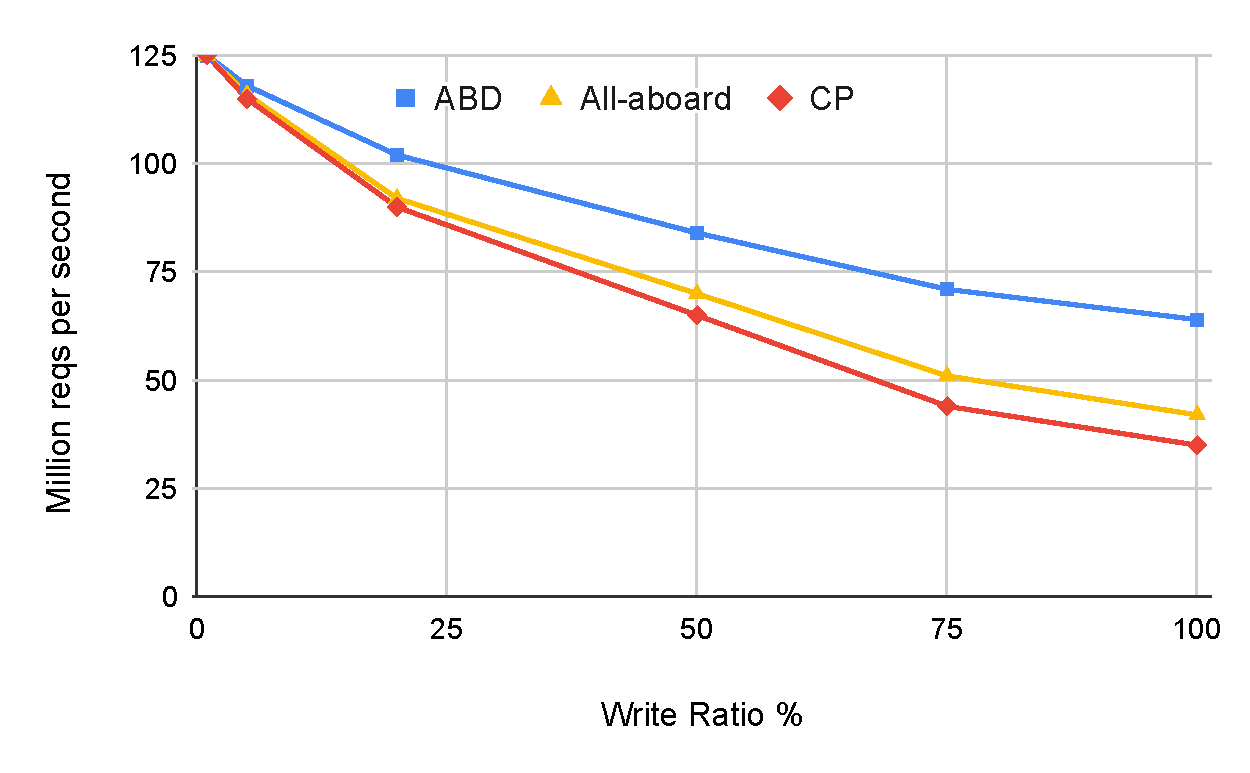
\includegraphics[width=0.4\textwidth]{1_figures/abd-ab-cp.pdf}
%   \vspace{-1.5em}
  \caption{Throughput vs write ratio for ABD, All-aboard \& CP}
%   \vspace{-1.5em}
  \label{fig:abd-ab-cp}
\end{figure}

\beginbsec{Performance}
Firstly, from \figref{fig:single-thr}, we observe that CP has the lowest single-threaded performance. This is because of the extremely high work-per-request ratio required in CP, as explained in \secref{sec:tax:dpko}. However,  CP is thread-scalable and well load balanced, enjoying a 10x improvement when multi-threaded (\figref{fig:write-all}) outperforming ZAB, MP and Derecho and matching CHT.

The All-aboard optimization reduces CP's high work-per-request but not completely.
This is why All-aboard is the second worse protocol when single-threaded.
Note that All-aboard has a significantly higher work-per-request ratio than Hermes and ABD, which also require two broadcast rounds. 
This highlights the fact that simply using the number of broadcast rounds as a metric to gauge performance is not sufficient. We need to factor in the size of the messages and the responses along with the complexity to create them.


Similarly to CP, All-aboard scales very well (10x) when multi-threaded, outperforming CP, CHT and the total order protocols.
Recall from \secref{sec:fail} that CP and All-aboard are the only two protocols (out of the \pnum) that can perform conditional writes while remaining available in the event of a failure. Therefore, for those keen on offering high availability, All-aboard comprises a great candidate, as it can also provide reasonably high performance.


ABD also offers the same levels of availability, but it is the only protocol out of the \pnum~that cannot perform conditional writes.
This simplification affords ABD a significantly lower work-per-request ratio than CP and All-aboard, which is why ABD outperforms CP and All-aboard both single-threaded and multi-threaded.
\figref{fig:abd-ab-cp} compares ABD, CP and All-aboard, varying the write ratio. Notably the read throughput is equal for all three, as they all implement ABD-reads. However, as the write ratio increases, ABD outperforms the other two due to its lower work-per-request ratio for writes.
Therefore, ABD comprises a great candidate, in cases where high availability is required and simple writes will suffice (as opposed to conditional writes).

\figref{fig:hr-cht-abd} compares ABD with Hermes (and CHT-mcast). Even though ABD is within a close distance in the write throughput, there is a big gap in the read throughput, demonstrating the cost of high availability. Specifically, Hermes mandates that every write reaches every node. In doing so, it concedes that all nodes must block on a failure (discussed in \secref{sec:fail}). However, it takes advantage of this concession in both reads and writes. In reads, by enabling them to execute locally, leveraging that all nodes have received the latest committed write. And in writes, by accelerating their operation, leveraging that a node that performs a write, has received all concurrent, conflicting writes.

This renders Hermes the better performing protocol out of all \pnum, making it an ideal candidate, for those who can afford an unavailability period in case of a failure.




\begin{comment}
\subsection{Hardware Multicast}\label{sec:ev:mcast}
Here we will discuss why the multicast primitive provides a 3x benefit for CHT, but no more than 5\% for the rest of the protocols.
The reason is that the multicast only relieves the send side of a broadcast.
% Using the hardware multicast primitive provides a 3x benefit for CHT. The benefit for the rest of the protocols is very small, typically around 5\%.
Specifically, on a multicast, one packet is sent to the switch instead of N (assuming N receipients). The switch then replicates the packet N times, propagating it to all recipients. Without using the multicast primitive, the sender must send N packets.
Let us use \figref{fig:mcast}, to investigate how multicasting affects CHT and Hermes.

\figref{fig:mcast} provides a pictorial view of the usage of the send and receive bandwidth for CHT, CHT-mcast, Hermes and Hermes-mcast. Firstly note that the figure does not provide a precise view of the measurements. Rather it illustrates a rough approximation that will help us explain why multicast is helpful in certain scenarios. To simplify further, in this discussion we will assume that smart-acks and smart-commits consume zero-bandwidth.

In \figref{fig:mcast}a, we see that the CHT leader uses up all of its send bandwidth. The leader utilizes a small fraction of its receive bandwidth receiving followers' writes.
% that are steered to it from the followers.
The receive side of the follower is not well utilized, because it only receives $1 / N$ of the messages sent by the leader (assuming an N-side deployment). The send side of the follower is used only to propagate writes to the leader. 

In \figref{fig:mcast}b we see how CHT is affected when using the multicast.
Leader's send side is still saturated, but now each packet is only sent once. Therefore, now the leader sends N times as many distinct packets.
Each follower now receives all the packets that the leader sends, because each packet is getting replicated at the switch and sent to all followers. Thus the follower's receive bandwidth is also saturated. Note that the send side of the follower is also increased, as the follower now propagates more packets to the leader. For that reason, the leader's receive side is saturated too.

Note the key insight: CHT-mcast improves upon CHT because in CHT the follower's receive side is underutilized. This allows us to leverage the leeway created by the multicast at the leader's send side by sending more packets to the followers. Had the follower's receive side not been underutilized, the multicast would simply reduce the utilization of the leader's send side.

This is exactly what happens with Hermes and Hermes-mcast in \figref{fig:mcast}c and d. In Hermes, all nodes utilize both the send and receive bandwidth symmetrically. Therefore, when multicast
is employed, the leeway created at the send side cannot be leveraged, because no node can receive any more packets.

To understand why CHT-mcast can match the performance of Hermes (or Hermes-mcast), consider the send bandwidth of the leader of CHT-mcast and the send bandwidth of a node in Hermes-mcast. Specifically, each Hermes-mcast node receives multicasts from the rest $N-1$ nodes. Therefore, each node can use up to $1/N-1$ of its send bandwidth. 
Therefore, all $N$ Hermes-mcast nodes use $N/N-1$ of one node's send bandwidth to multicast new writes.
Comparing that with CHT-mcast, we can infer that Hermes-mcast can in theory be only $N/N-1$ times better than CHT-mcast. For instance in our 5-node deployment, Hermes should be able to achieve a 25\% increase over CHT-mcast. 
Furthermore, in theory Hermes and Hermes-mcast should have the same performance.

\figref{fig:hr-cht-abd}, shows that in practice, because Hermes does not manage to fully saturate its send bandwidth, CHT-mcast and Hermes (without multicast) have almost identical behaviour for all write ratios. Finally, the write throughput of Hermes-mcast (94 M.reqs/s) is around 10\% better than CHT-mcast.


\begin{figure}[t]
  \centering
  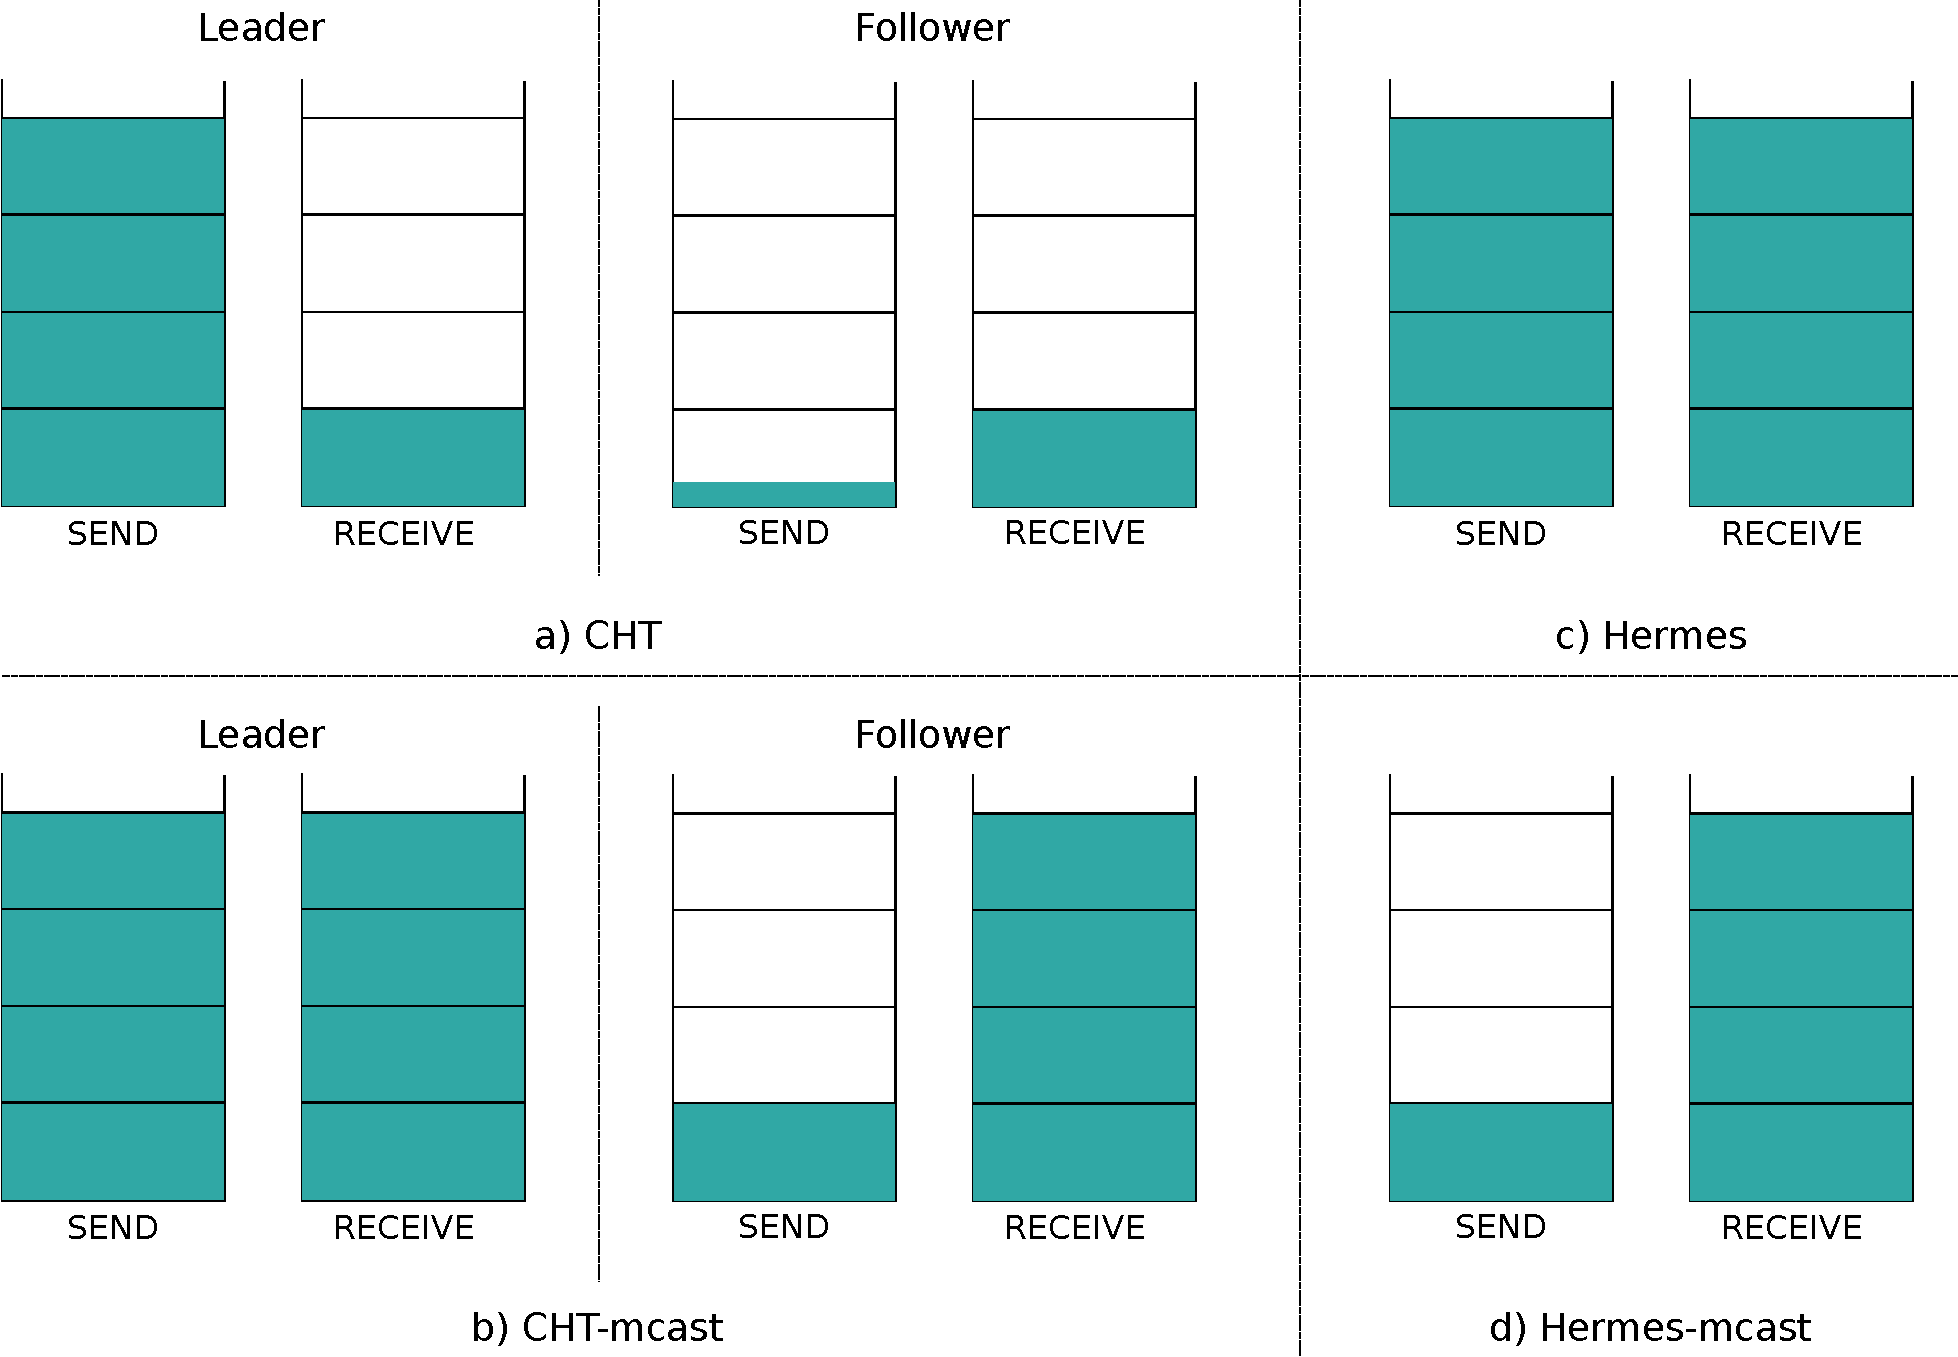
\includegraphics[width=0.47\textwidth]{1_figures/mcast.pdf}
%   \vspace{-0.5em}
  \caption{An illustration of the send and receive bandwidth of CHT, CHT-mcast, Hermes and Hermes-mcast}
%   \vspace{-1.5em}
  \label{fig:mcast}
\end{figure}
% Therefore, in a load balanced scenario, where each machine sends out as much data as it receives, using the multicast will not help even if the bottleneck is at the network. Because the pressure is relieved \emph{only} on the send side. The nodes will keep receiving the same amount of packets.

% In CHT's case, for each write the leader must do a broadcast, \ie  send N-1 unicasts.
% In return it only receives small smart-acks. 
% The followers only receive one message per write.
% Therefore the send side of the leader is substantially more loaded. As a result, CHT scales only up to five threads (\ie workers), which are enough to saturate the leader's send side of our 56 Gbit NIC. Beyond that the write throughput flatlines at 28 M.reqs/s.

% When enabling multicast, the leader's send side gets relieved and the throughput scales up to 85 M.reqs/s. Note however, that CHT-mcast still does not utilize all available resources: followers' send side are still underutilized. How does it then match Hermes' performance?
% CHT-mcast sends one message per write where Hermes sends N-1 (with N nodes). And thus Hermes needs to utilize all nodes' send bandwidth, to provide the same throughput. However, Hermes cannot utilize the multicast: even when it uses it the send side of all nodes get relieved but the receive side remains jammed.



% only needs to send one message per write.
% The followers each receive one message. The protocol still does not utilize all available resources: leader's receive side and followers' send side are still underutilized. How can then CHT-mcast match Hermes, which uses all resources?

% Compare that to Hermes, where each write 


%  This is why in our results we only use multicast for CHT.
\end{comment}
\begin{comment}
\beginbsec{Writes}
ABD assumes that each object is stored along with a unique identifier of its last write. Most commonly that is a Lamport logical clock~\cite{Lamport:1978}.
We will refer to that unique identifier as timestamp (TS).
A write to key $K$ requires two broadcast rounds. 
A first lightweight round learns the TSes stored in a majority of remote nodes. The writer uses the remote TSes, to create a new larger TS and tag its write, which it broadcasts in its second round.
The write can commit upon receiving a majority of acks (implemented with \odlib~smart-acks).
% The first round requests remote nodes to tell it their locally stored TS for $K$. The writer waits only for a majority of responses (including its own). By the end of the round, the writer knows what is the latest write (by its TS) that has been committed in a majority of replicas. This is because, any write that has been applied to a majority of replicas, must overlap with he majority of responses that the writer received.

\beginbsec{Reads}
Reads perform one broadcast round and then an optional second round.
The first round broadcasts the locally stored TS and asks remote nodes if they store the same TS, a lower one or a higher. If replicas store a higher TS, they respond with both the TS and the value. The read gathers a majority of replies.
If the read cannot infer that a majority of replicas stores the value that the read wishes to return, then it performs a second round, which is identical to the write's second round. The second round is not necessary in more than 99\% of the reads.
\end{comment}
\begin{comment}
Notably, CP has not been widely used to perform conditional writes. This is because in Lamport's original paper it was not described how to run CP repeatedly, but we must be able to modify the same object multiple times. Rather Lamport suggested that CP can be executed once to establish a leader which can then make all decisions (\ie Multi-Paxos).

However, Lamport in his original paper did explain that it is possible to run CP without a log over a KVS. Recently, there have been a few proposals~\cite{Skrzypczak:2020, Rystsov:2018} that combine this observation with enhancements to CP so that it can run repeatedly in order to support conditional writes. 
In fact, Gavrielatos \etal~\cite{V:2020} showed that CP can be competitive, if multi-threaded, however they never revealed any details on how it can be so.

In this work, we replicate the results of~\cite{V:2020}, over \odlib~and we enhance it with  the All-Aboard optimization, sketched in Howard's thesis~\cite{Howard:2019}. % 2) the carstamps proposed by Burke \etal~\cite{Burke:2020}, so that it can be combined with ABD reads and writes.
Notably, the specification of the enhancements required for CP (to run it  repeatedly) and All-aboard are out of the scope of this paper. However, as a companion to this paper, we will also publish the full specification and implementation description of both our CP and All-aboard. 
%The specification safely extends CP so that it can be executed repeatedly, and it elaborates on multi-threading CP.
Below we provide a brief description of the implementation of writes in CP and All-aboard.

\beginbsec{Writes}
CP requires three broadcast rounds to complete a write: propose, accept and commit. Upon receiving any of the three messages, a worker locks the corresponding key-value pair, it examines its CP-related metadata (\eg its timestamps), it modifies it accordingly and it replies. 
Proposes and accepts can be acknowledged (acked) or negatively-acked (nacked).
Commits require no response.
Upon receiving a majority of acks for a propose, the worker, that coordinates the write, broadcasts accepts. Upon a majority of acks to an accept the write can be committed. 

All-aboard omits the first round (proposes) and directly broadcasts accepts.
If \emph{all} remote nodes ack the accept, then the write can be committed, and commits are broadcast. If the accept does not manage to gather all acks, either because of a nack or because of a slow node, then it starts over running full CP. In our setting, All-aboard is successful in more than 99\% of writes.

% \beginbsec{Reads}
% We implement reads through a modified version of ABD reads. ABD reads require one broadcast round with an optional second. ABD assumes each key is stored along with its The first round broadcastsasks remote nodes if they are storing the same version , the first to read the version of the key from a majority of nodes.


\subsubsection{Performance}
% \begin{figure}[t]
  \centering
  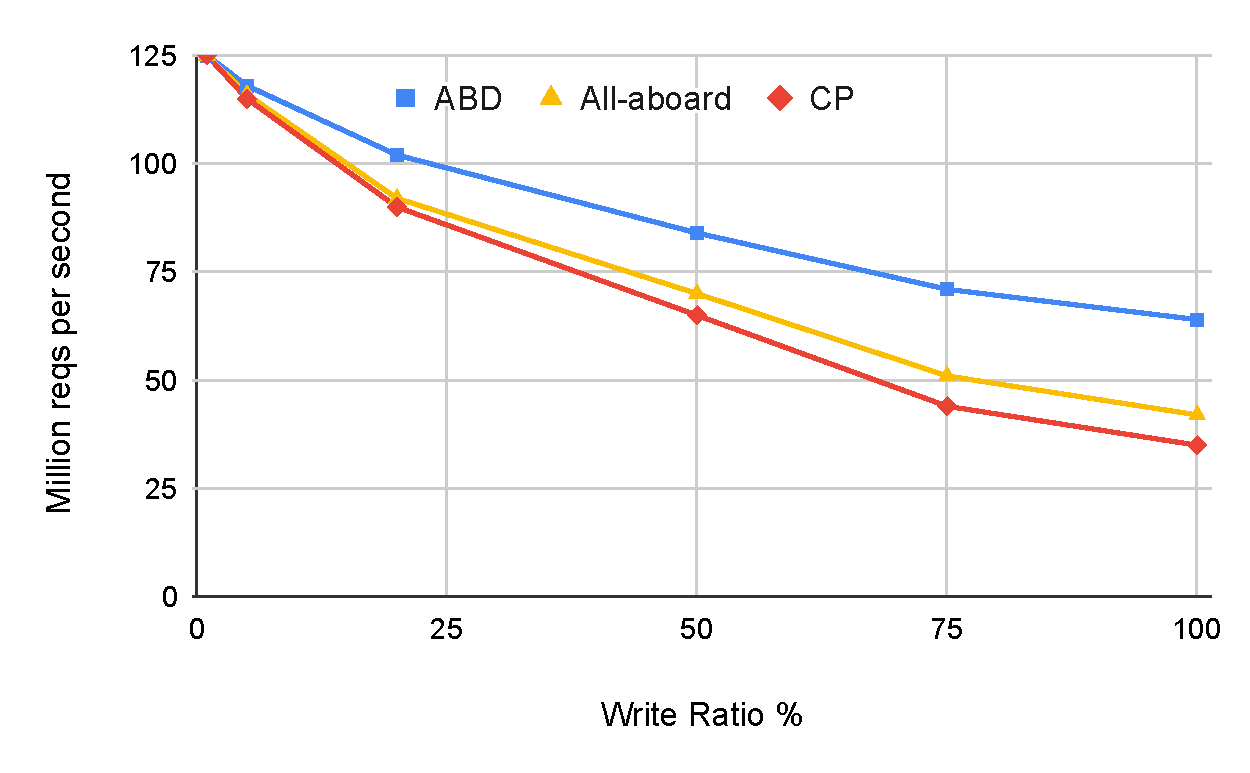
\includegraphics[width=0.4\textwidth]{1_figures/abd-ab-cp.pdf}
%   \vspace{-1.5em}
  \caption{Throughput vs write ratio for ABD, All-aboard \& CP}
%   \vspace{-1.5em}
  \label{fig:abd-ab-cp}
\end{figure}
% \begin{figure}[t]
  \centering
  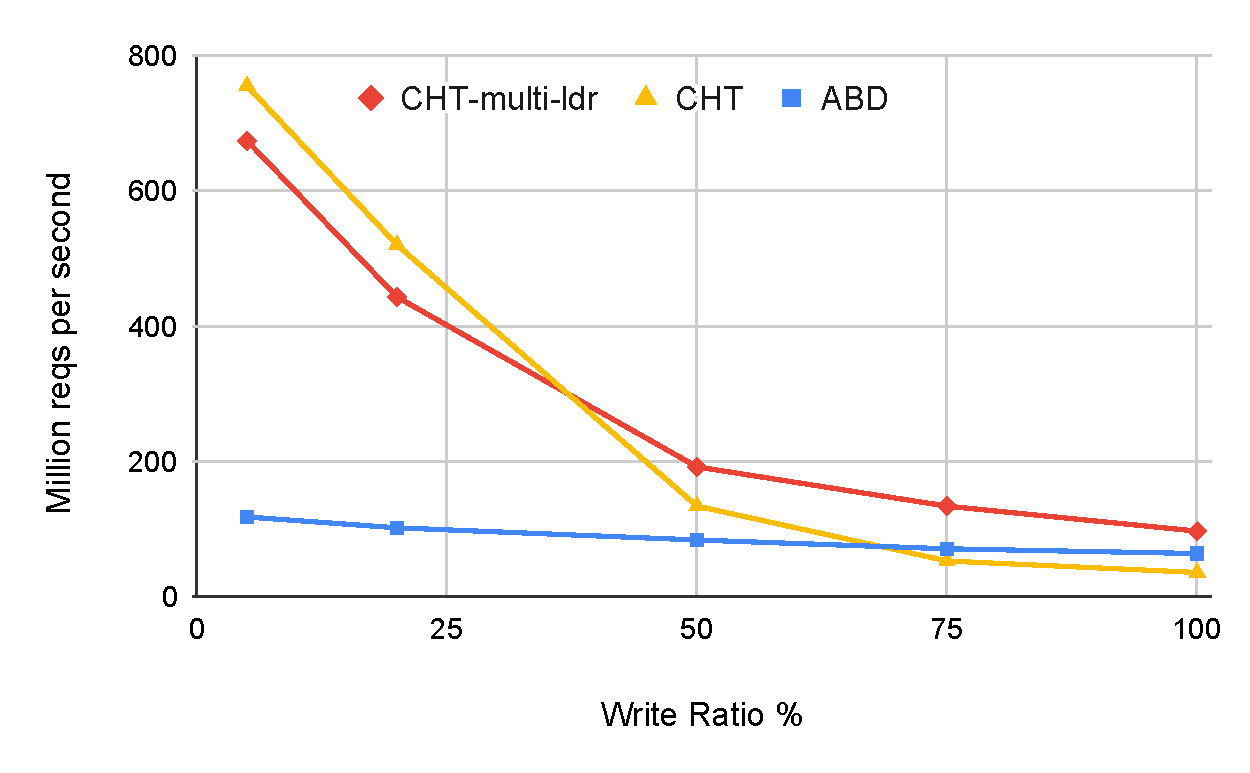
\includegraphics[scale=0.4]{1_figures/chtml-cht-abd.pdf}
%   \vspace{-0.5em}
  \caption{Throughput of CHT-multi-ldr, CHT \& ABD, varying the write ratio from 1\% to 100\%}
%   \vspace{-1.5em}
  \label{fig:cht-cht-abd}
\end{figure}
Firstly, from Figures~\ref{fig:write-all} and \ref{fig:single-thr}, we can see that all three protocols scale reasonably well with more threads. 
%And all three are load balanced as all nodes coordinate their own writes.
In fact, CP and All-aboard are the worst performing protocols when single-threaded.
This is because both protocols must do a lot of work to complete a request.
Notably, CP and All-aboard provide a unique design point as the only protocols that can execute a conditional write and remain available in the event of the fault. 
This is the equivalent of asynchronous consensus.
The cost of this is the very high work-per-request ratio.
All-aboard is very attractive design point for a scenario, where 1) availability is the most important concern 2) conditional writes are required and 3) multi-threading is possible.
If simple writes will do, then ABD is the best option.
% For instance the second round of ABD is 48 bytes, while an accept of CP or All-aboard is 76B.

\figref{fig:abd-ab-cp} shows the throughput of ABD, CP and All-aboard. 
ABD cannot solve consensus, but is significantly simpler than CP and All-aboard, which allows it to perform much better in high write ratios.% both when single-threaded and multi-threaded.
However, in low write ratios it's still outperformed when compared with protocols with local reads that are willing to trade-off availability guarantees for performance.
\figref{fig:cht-cht-abd} depicts just that comparing ABD For instance, with CHT and CHT-multi-ldr, both of which perform reads locally.
% Their read-only throughput is the same, as they all use ABD reads.
% Note that even though ABD and All-aboard both require 2 broadcast rounds for their writes, ABD significantly outperforms All-aboard for high write ratios.
% The reason is that the ABD protocol is substantially simpler and the messages are much smaller. For instance, the second round of ABD is 48 bytes, while an accept is 76B. This is the cost of conditional writes, which All-aboard can execute, but ABD cannot.

% Furthermore, all three protocols are significantly outperformed in low write ratios by protocols that can offer local reads. This is depicted in \figref{fig:hr-dr-cp}, where CP is compared to Hermes and Derecho.
% The reads are implemented identically in all three protocols (with ABD reads). In addition, these are the only three protocols 
% A nack to a propose or accept always includes the reason why can have a variety of dif
\end{comment}
\begin{comment}


\subsubsection{Writes}
\figref{fig:write-all} shows the throughput of all protocols in million requests per second (M.reqs/s) for a write-only setting. Firstly, note that there is a protocol called CHT-mcast. This is the CHT protocol (not CHT-multi-ldr), when the hardware multicast is enabled. Secondly note that that all protocols except ABD, can implement conditional writes (\ie RMWs).


Based on \figref{fig:write-all}, we group protocols into low and high-performers and provide a brief explanation in order to relate them.

\beginbsec{Low-performers}
 ZAB, Multi-Paxos and Derecho are the worst performers. The reason is they lack thread scalability, due to the fact that they must create an order among all writes.
Classic Paxos and its optimization All-aboard Paxos are performing better but still suffer from a very high work-per-request index that is fundamental to their internal complexity.
CHT is thread scalable and has a relatively low work-per-request ratio but does not manage to balance the load: it is bottlenecked by the send bandwidth of the single leader.

\beginbsec{High-performers}
All of the high-performers are mostly thread scalable, load balanced and with a low work-per-request. Hermes serves here as the baseline, as it is completely load balanced, perfectly thread-scalable and has the lowest work-per-request.  
ABD, CHT-multi-leader and CHT-mcast have a bit higher work-per-request than the rest. ABD in order to ensure perfect availability and CHT-multi-leader and CHT-mcast in order to steer writes to the leader.
Finally, CRAQ is not perfectly load balanced as the tail node does not equally participate in the load.  

\subsubsection{Reads}
\figref{fig:write-5per} shows the throughput in M.reqs/s for a read-mostly workload (5\% writes).
First note that both the x-axis and the y-axis are different from \figref{fig:write-all}.
Secondly, note that ZAB and Derecho offer Sequential Consistency, while the rest offer Linearizability. As before, ABD writes cannot be conditional (\ie RMWs).

Operationally there are three groups. Multi-Paxos steers reads to the leader node.  CP, All-aboard and ABD use ABD reads. The rest all use local reads. 

Multi-Paxos performance suffers as its the only non-thread-scalable protocol that does not perform reads locally.  
CP, All-aboard and ABD all come close to the maximum ABD-read throughput (125 M.reqs/s). 

% two issues: firstly the work-per-request is the highest among all protocols we evaluate. This however is balanced with the high availability they offer. Both protocols can continue operating without interruption in the face of a failure. The other problem is that CP and ABP are not perfectly thread-scalable. Because of the 

% \begin{figure}[t]
  \centering
  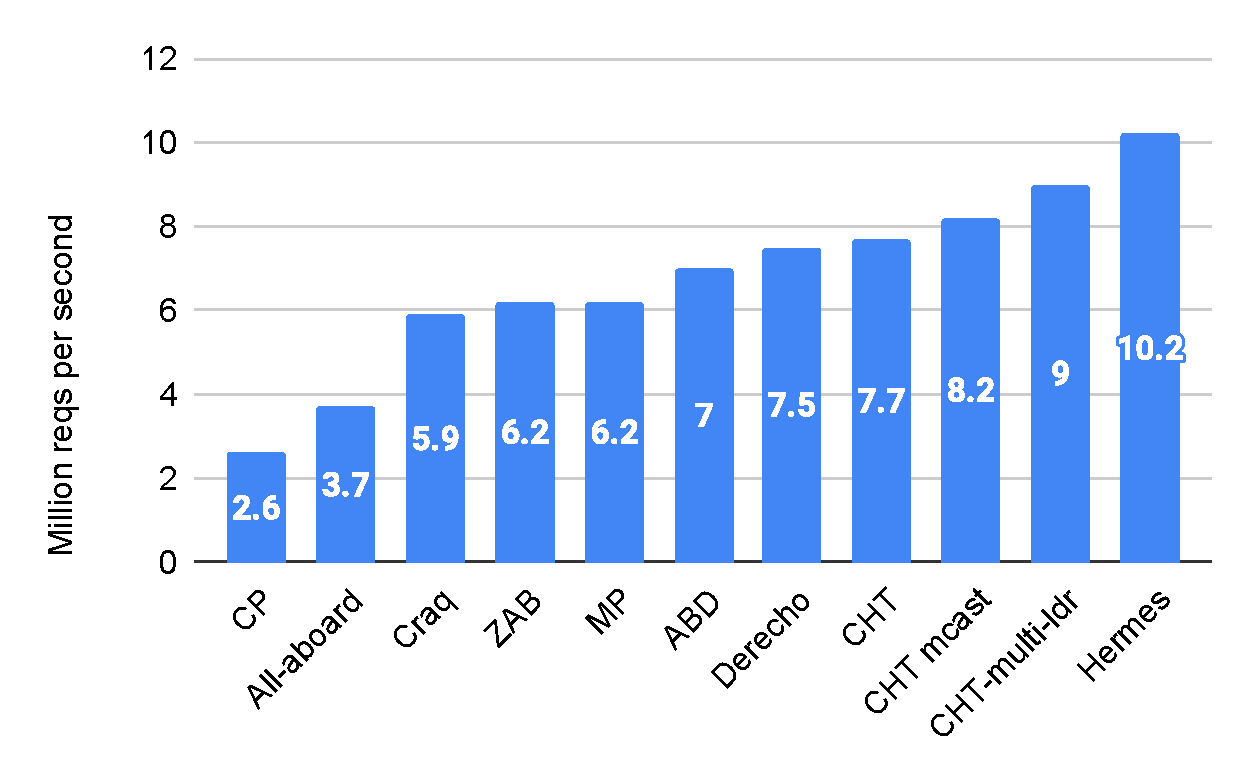
\includegraphics[scale=0.4]{1_figures/single-thread.pdf}
%   \vspace{-0.5em}
  \caption{Single-threaded write throughput of all protocols}
%   \vspace{-1.5em}
  \label{fig:single-thr}
\end{figure}
% \begin{figure}[t]
  \centering
  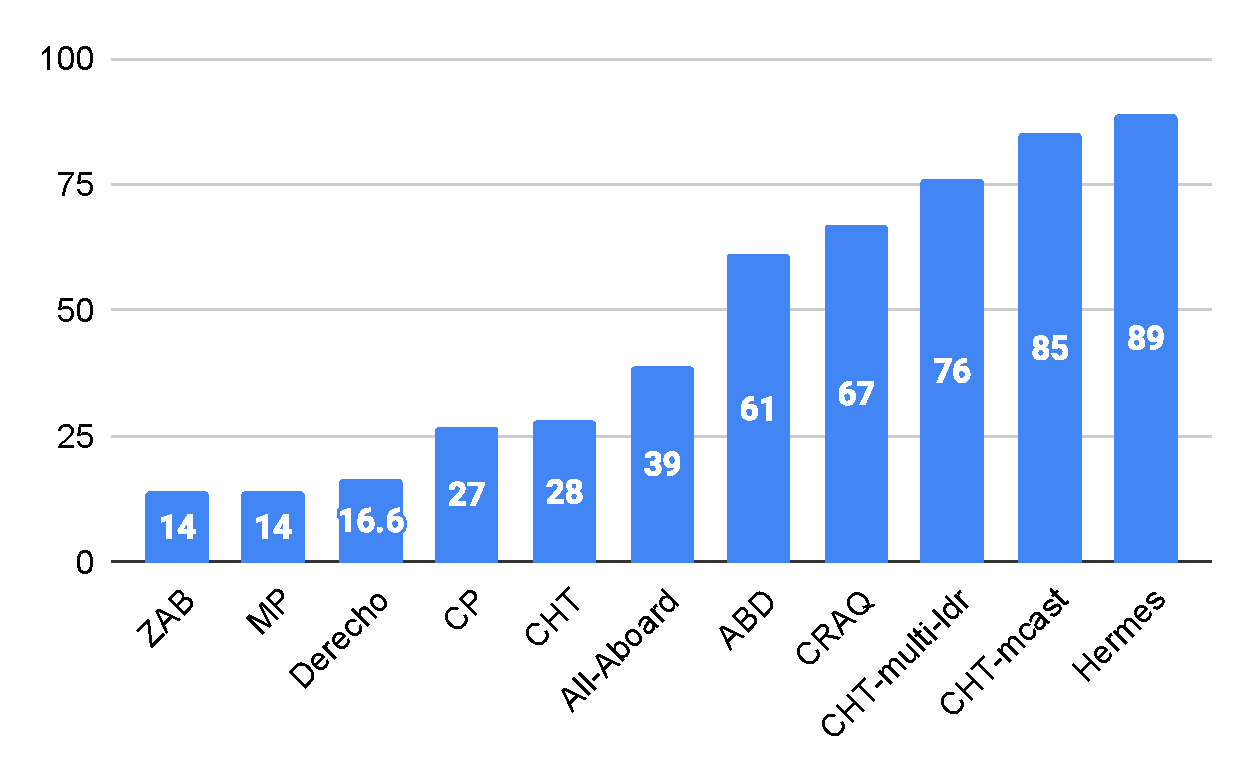
\includegraphics[scale=0.4]{1_figures/Write-only-chart.pdf}
%   \vspace{-0.5em}
  \caption{Write throughput of all protocols [5 nodes]}
%   \vspace{-1.5em}
  \label{fig:write-all}
\end{figure}
% \begin{figure}[t]
  \centering
  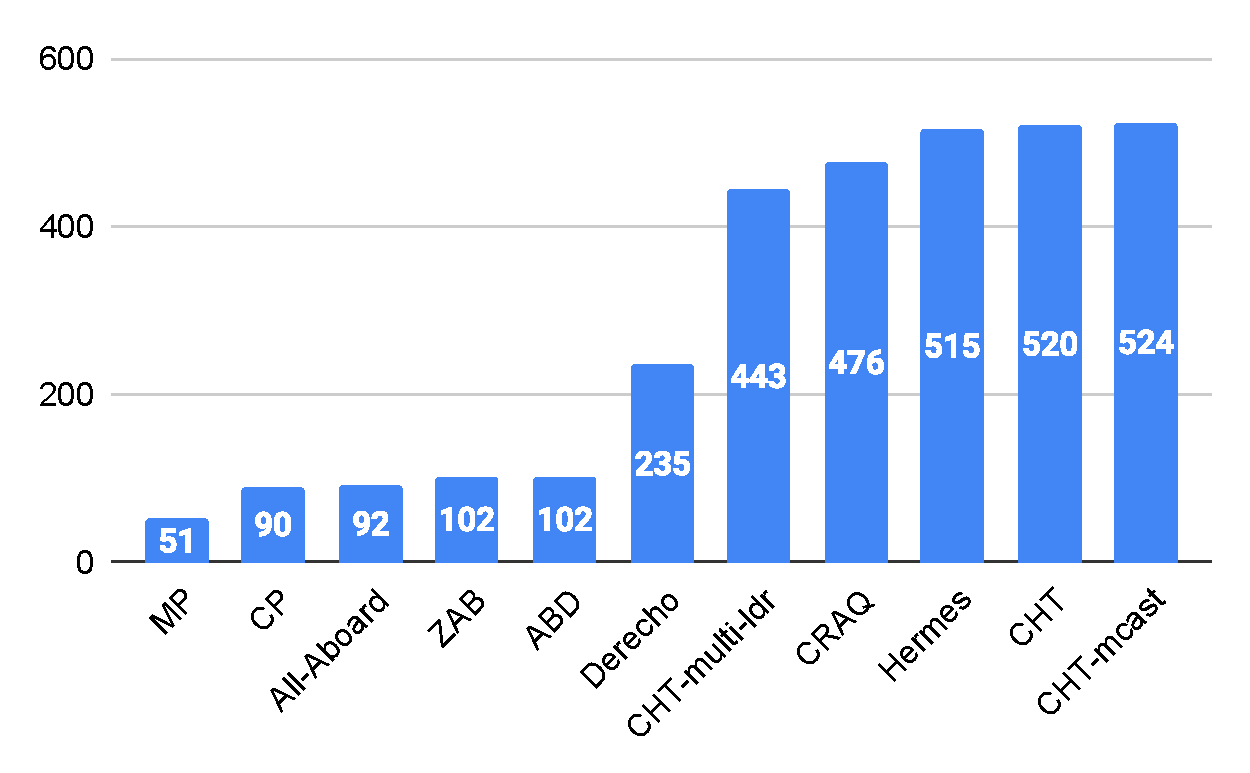
\includegraphics[scale=0.4]{1_figures/5perc-writes.pdf}
%   \vspace{-0.5em}
  \caption{Throughput of all protocols at 95\% reads}
%   \vspace{-1.5em}
  \label{fig:5perc}
\end{figure}


\end{comment}